\documentclass[lettersize,journal]{IEEEtran}
%%%%%%%%%%%---SETME-----%%%%%%%%%%%%%
%replace @@ with the submission number submission site.
\newcommand{\thiswork}{INF$^2$\xspace}
%%%%%%%%%%%%%%%%%%%%%%%%%%%%%%%%%%%%


%\newcommand{\rev}[1]{{\color{olivegreen}#1}}
\newcommand{\rev}[1]{{#1}}


\newcommand{\JL}[1]{{\color{cyan}[\textbf{\sc JLee}: \textit{#1}]}}
\newcommand{\JW}[1]{{\color{orange}[\textbf{\sc JJung}: \textit{#1}]}}
\newcommand{\JY}[1]{{\color{blue(ncs)}[\textbf{\sc JSong}: \textit{#1}]}}
\newcommand{\HS}[1]{{\color{magenta}[\textbf{\sc HJang}: \textit{#1}]}}
\newcommand{\CS}[1]{{\color{navy}[\textbf{\sc CShin}: \textit{#1}]}}
\newcommand{\SN}[1]{{\color{olive}[\textbf{\sc SNoh}: \textit{#1}]}}

%\def\final{}   % uncomment this for the submission version
\ifdefined\final
\renewcommand{\JL}[1]{}
\renewcommand{\JW}[1]{}
\renewcommand{\JY}[1]{}
\renewcommand{\HS}[1]{}
\renewcommand{\CS}[1]{}
\renewcommand{\SN}[1]{}
\fi

%%% Notion for baseline approaches %%% 
\newcommand{\baseline}{offloading-based batched inference\xspace}
\newcommand{\Baseline}{Offloading-based batched inference\xspace}


\newcommand{\ans}{attention-near storage\xspace}
\newcommand{\Ans}{Attention-near storage\xspace}
\newcommand{\ANS}{Attention-Near Storage\xspace}

\newcommand{\wb}{delayed KV cache writeback\xspace}
\newcommand{\Wb}{Delayed KV cache writeback\xspace}
\newcommand{\WB}{Delayed KV Cache Writeback\xspace}

\newcommand{\xcache}{X-cache\xspace}
\newcommand{\XCACHE}{X-Cache\xspace}


%%% Notions for our methods %%%
\newcommand{\schemea}{\textbf{Expanding supported maximum sequence length with optimized performance}\xspace}
\newcommand{\Schemea}{\textbf{Expanding supported maximum sequence length with optimized performance}\xspace}

\newcommand{\schemeb}{\textbf{Optimizing the storage device performance}\xspace}
\newcommand{\Schemeb}{\textbf{Optimizing the storage device performance}\xspace}

\newcommand{\schemec}{\textbf{Orthogonally supporting Compression Techniques}\xspace}
\newcommand{\Schemec}{\textbf{Orthogonally supporting Compression Techniques}\xspace}



% Circular numbers
\usepackage{tikz}
\newcommand*\circled[1]{\tikz[baseline=(char.base)]{
            \node[shape=circle,draw,inner sep=0.4pt] (char) {#1};}}

\newcommand*\bcircled[1]{\tikz[baseline=(char.base)]{
            \node[shape=circle,draw,inner sep=0.4pt, fill=black, text=white] (char) {#1};}}

\ifCLASSINFOpdf
            \else
                  \fi

\hyphenation{op-tical net-works semi-conduc-tor}

\begin{document}
 
\title{Securing 5G Bootstrapping: A Two-Layer\\ IBS Authentication Protocol}
 
\author{Yilu~Dong,
        Rouzbeh~Behnia,
        Attila~A.~Yavuz,
        and~Syed~Rafiul~Hussain,~\IEEEmembership{Member,~IEEE}}

\maketitle

\begin{abstract}
The lack of authentication during the initial bootstrapping phase between cellular devices and base stations allows attackers to deploy fake base stations and send malicious messages to the devices. These attacks have been a long-existing problem in cellular networks, enabling adversaries to launch denial-of-service (DoS), information leakage, and location-tracking attacks. While some defense mechanisms are introduced in 5G, (e.g., encrypting user identifiers to mitigate IMSI catchers), the initial communication between devices and base stations remains unauthenticated, leaving a critical security gap. To address this, we propose \scheme{}, a novel and efficient two-layer identity-based signature scheme designed for seamless integration with existing cellular protocols. We implement \scheme{} on an open-source 5G stack and conduct a comprehensive performance evaluation against alternative solutions. Compared to the state-of-the-art \texttt{Schnorr-HIBS}, \scheme{} reduces attack surfaces, enables fine-grained lawful interception, and achieves 2x speed in verification, making it a practical solution for securing 5G base station authentication.
\end{abstract}

\begin{IEEEkeywords}
Cellular Networks, Fake Base Station Attacks, Identity-Based Signatures, Authentication Protocol.  
\end{IEEEkeywords}

\IEEEpeerreviewmaketitle

\hfill  
 
\hfill January 30, 2025

\section{Introduction}
\section{Introduction}
\label{sec:introduction}
The business processes of organizations are experiencing ever-increasing complexity due to the large amount of data, high number of users, and high-tech devices involved \cite{martin2021pmopportunitieschallenges, beerepoot2023biggestbpmproblems}. This complexity may cause business processes to deviate from normal control flow due to unforeseen and disruptive anomalies \cite{adams2023proceddsriftdetection}. These control-flow anomalies manifest as unknown, skipped, and wrongly-ordered activities in the traces of event logs monitored from the execution of business processes \cite{ko2023adsystematicreview}. For the sake of clarity, let us consider an illustrative example of such anomalies. Figure \ref{FP_ANOMALIES} shows a so-called event log footprint, which captures the control flow relations of four activities of a hypothetical event log. In particular, this footprint captures the control-flow relations between activities \texttt{a}, \texttt{b}, \texttt{c} and \texttt{d}. These are the causal ($\rightarrow$) relation, concurrent ($\parallel$) relation, and other ($\#$) relations such as exclusivity or non-local dependency \cite{aalst2022pmhandbook}. In addition, on the right are six traces, of which five exhibit skipped, wrongly-ordered and unknown control-flow anomalies. For example, $\langle$\texttt{a b d}$\rangle$ has a skipped activity, which is \texttt{c}. Because of this skipped activity, the control-flow relation \texttt{b}$\,\#\,$\texttt{d} is violated, since \texttt{d} directly follows \texttt{b} in the anomalous trace.
\begin{figure}[!t]
\centering
\includegraphics[width=0.9\columnwidth]{images/FP_ANOMALIES.png}
\caption{An example event log footprint with six traces, of which five exhibit control-flow anomalies.}
\label{FP_ANOMALIES}
\end{figure}

\subsection{Control-flow anomaly detection}
Control-flow anomaly detection techniques aim to characterize the normal control flow from event logs and verify whether these deviations occur in new event logs \cite{ko2023adsystematicreview}. To develop control-flow anomaly detection techniques, \revision{process mining} has seen widespread adoption owing to process discovery and \revision{conformance checking}. On the one hand, process discovery is a set of algorithms that encode control-flow relations as a set of model elements and constraints according to a given modeling formalism \cite{aalst2022pmhandbook}; hereafter, we refer to the Petri net, a widespread modeling formalism. On the other hand, \revision{conformance checking} is an explainable set of algorithms that allows linking any deviations with the reference Petri net and providing the fitness measure, namely a measure of how much the Petri net fits the new event log \cite{aalst2022pmhandbook}. Many control-flow anomaly detection techniques based on \revision{conformance checking} (hereafter, \revision{conformance checking}-based techniques) use the fitness measure to determine whether an event log is anomalous \cite{bezerra2009pmad, bezerra2013adlogspais, myers2018icsadpm, pecchia2020applicationfailuresanalysispm}. 

The scientific literature also includes many \revision{conformance checking}-independent techniques for control-flow anomaly detection that combine specific types of trace encodings with machine/deep learning \cite{ko2023adsystematicreview, tavares2023pmtraceencoding}. Whereas these techniques are very effective, their explainability is challenging due to both the type of trace encoding employed and the machine/deep learning model used \cite{rawal2022trustworthyaiadvances,li2023explainablead}. Hence, in the following, we focus on the shortcomings of \revision{conformance checking}-based techniques to investigate whether it is possible to support the development of competitive control-flow anomaly detection techniques while maintaining the explainable nature of \revision{conformance checking}.
\begin{figure}[!t]
\centering
\includegraphics[width=\columnwidth]{images/HIGH_LEVEL_VIEW.png}
\caption{A high-level view of the proposed framework for combining \revision{process mining}-based feature extraction with dimensionality reduction for control-flow anomaly detection.}
\label{HIGH_LEVEL_VIEW}
\end{figure}

\subsection{Shortcomings of \revision{conformance checking}-based techniques}
Unfortunately, the detection effectiveness of \revision{conformance checking}-based techniques is affected by noisy data and low-quality Petri nets, which may be due to human errors in the modeling process or representational bias of process discovery algorithms \cite{bezerra2013adlogspais, pecchia2020applicationfailuresanalysispm, aalst2016pm}. Specifically, on the one hand, noisy data may introduce infrequent and deceptive control-flow relations that may result in inconsistent fitness measures, whereas, on the other hand, checking event logs against a low-quality Petri net could lead to an unreliable distribution of fitness measures. Nonetheless, such Petri nets can still be used as references to obtain insightful information for \revision{process mining}-based feature extraction, supporting the development of competitive and explainable \revision{conformance checking}-based techniques for control-flow anomaly detection despite the problems above. For example, a few works outline that token-based \revision{conformance checking} can be used for \revision{process mining}-based feature extraction to build tabular data and develop effective \revision{conformance checking}-based techniques for control-flow anomaly detection \cite{singh2022lapmsh, debenedictis2023dtadiiot}. However, to the best of our knowledge, the scientific literature lacks a structured proposal for \revision{process mining}-based feature extraction using the state-of-the-art \revision{conformance checking} variant, namely alignment-based \revision{conformance checking}.

\subsection{Contributions}
We propose a novel \revision{process mining}-based feature extraction approach with alignment-based \revision{conformance checking}. This variant aligns the deviating control flow with a reference Petri net; the resulting alignment can be inspected to extract additional statistics such as the number of times a given activity caused mismatches \cite{aalst2022pmhandbook}. We integrate this approach into a flexible and explainable framework for developing techniques for control-flow anomaly detection. The framework combines \revision{process mining}-based feature extraction and dimensionality reduction to handle high-dimensional feature sets, achieve detection effectiveness, and support explainability. Notably, in addition to our proposed \revision{process mining}-based feature extraction approach, the framework allows employing other approaches, enabling a fair comparison of multiple \revision{conformance checking}-based and \revision{conformance checking}-independent techniques for control-flow anomaly detection. Figure \ref{HIGH_LEVEL_VIEW} shows a high-level view of the framework. Business processes are monitored, and event logs obtained from the database of information systems. Subsequently, \revision{process mining}-based feature extraction is applied to these event logs and tabular data input to dimensionality reduction to identify control-flow anomalies. We apply several \revision{conformance checking}-based and \revision{conformance checking}-independent framework techniques to publicly available datasets, simulated data of a case study from railways, and real-world data of a case study from healthcare. We show that the framework techniques implementing our approach outperform the baseline \revision{conformance checking}-based techniques while maintaining the explainable nature of \revision{conformance checking}.

In summary, the contributions of this paper are as follows.
\begin{itemize}
    \item{
        A novel \revision{process mining}-based feature extraction approach to support the development of competitive and explainable \revision{conformance checking}-based techniques for control-flow anomaly detection.
    }
    \item{
        A flexible and explainable framework for developing techniques for control-flow anomaly detection using \revision{process mining}-based feature extraction and dimensionality reduction.
    }
    \item{
        Application to synthetic and real-world datasets of several \revision{conformance checking}-based and \revision{conformance checking}-independent framework techniques, evaluating their detection effectiveness and explainability.
    }
\end{itemize}

The rest of the paper is organized as follows.
\begin{itemize}
    \item Section \ref{sec:related_work} reviews the existing techniques for control-flow anomaly detection, categorizing them into \revision{conformance checking}-based and \revision{conformance checking}-independent techniques.
    \item Section \ref{sec:abccfe} provides the preliminaries of \revision{process mining} to establish the notation used throughout the paper, and delves into the details of the proposed \revision{process mining}-based feature extraction approach with alignment-based \revision{conformance checking}.
    \item Section \ref{sec:framework} describes the framework for developing \revision{conformance checking}-based and \revision{conformance checking}-independent techniques for control-flow anomaly detection that combine \revision{process mining}-based feature extraction and dimensionality reduction.
    \item Section \ref{sec:evaluation} presents the experiments conducted with multiple framework and baseline techniques using data from publicly available datasets and case studies.
    \item Section \ref{sec:conclusions} draws the conclusions and presents future work.
\end{itemize}

\section{Background}
\label{Background}
\section{Background}\label{sec:backgrnd}

\subsection{Cold Start Latency and Mitigation Techniques}

Traditional FaaS platforms mitigate cold starts through snapshotting, lightweight virtualization, and warm-state management. Snapshot-based methods like \textbf{REAP} and \textbf{Catalyzer} reduce initialization time by preloading or restoring container states but require significant memory and I/O resources, limiting scalability~\cite{dong_catalyzer_2020, ustiugov_benchmarking_2021}. Lightweight virtualization solutions, such as \textbf{Firecracker} microVMs, achieve fast startup times with strong isolation but depend on robust infrastructure, making them less adaptable to fluctuating workloads~\cite{agache_firecracker_2020}. Warm-state management techniques like \textbf{Faa\$T}~\cite{romero_faa_2021} and \textbf{Kraken}~\cite{vivek_kraken_2021} keep frequently invoked containers ready, balancing readiness and cost efficiency under predictable workloads but incurring overhead when demand is erratic~\cite{romero_faa_2021, vivek_kraken_2021}. While these methods perform well in resource-rich cloud environments, their resource intensity challenges applicability in edge settings.

\subsubsection{Edge FaaS Perspective}

In edge environments, cold start mitigation emphasizes lightweight designs, resource sharing, and hybrid task distribution. Lightweight execution environments like unikernels~\cite{edward_sock_2018} and \textbf{Firecracker}~\cite{agache_firecracker_2020}, as used by \textbf{TinyFaaS}~\cite{pfandzelter_tinyfaas_2020}, minimize resource usage and initialization delays but require careful orchestration to avoid resource contention. Function co-location, demonstrated by \textbf{Photons}~\cite{v_dukic_photons_2020}, reduces redundant initializations by sharing runtime resources among related functions, though this complicates isolation in multi-tenant setups~\cite{v_dukic_photons_2020}. Hybrid offloading frameworks like \textbf{GeoFaaS}~\cite{malekabbasi_geofaas_2024} balance edge-cloud workloads by offloading latency-tolerant tasks to the cloud and reserving edge resources for real-time operations, requiring reliable connectivity and efficient task management. These edge-specific strategies address cold starts effectively but introduce challenges in scalability and orchestration.

\subsection{Predictive Scaling and Caching Techniques}

Efficient resource allocation is vital for maintaining low latency and high availability in serverless platforms. Predictive scaling and caching techniques dynamically provision resources and reduce cold start latency by leveraging workload prediction and state retention.
Traditional FaaS platforms use predictive scaling and caching to optimize resources, employing techniques (OFC, FaasCache) to reduce cold starts. However, these methods rely on centralized orchestration and workload predictability, limiting their effectiveness in dynamic, resource-constrained edge environments.



\subsubsection{Edge FaaS Perspective}

Edge FaaS platforms adapt predictive scaling and caching techniques to constrain resources and heterogeneous environments. \textbf{EDGE-Cache}~\cite{kim_delay-aware_2022} uses traffic profiling to selectively retain high-priority functions, reducing memory overhead while maintaining readiness for frequent requests. Hybrid frameworks like \textbf{GeoFaaS}~\cite{malekabbasi_geofaas_2024} implement distributed caching to balance resources between edge and cloud nodes, enabling low-latency processing for critical tasks while offloading less critical workloads. Machine learning methods, such as clustering-based workload predictors~\cite{gao_machine_2020} and GRU-based models~\cite{guo_applying_2018}, enhance resource provisioning in edge systems by efficiently forecasting workload spikes. These innovations effectively address cold start challenges in edge environments, though their dependency on accurate predictions and robust orchestration poses scalability challenges.

\subsection{Decentralized Orchestration, Function Placement, and Scheduling}

Efficient orchestration in serverless platforms involves workload distribution, resource optimization, and performance assurance. While traditional FaaS platforms rely on centralized control, edge environments require decentralized and adaptive strategies to address unique challenges such as resource constraints and heterogeneous hardware.



\subsubsection{Edge FaaS Perspective}

Edge FaaS platforms adopt decentralized and adaptive orchestration frameworks to meet the demands of resource-constrained environments. Systems like \textbf{Wukong} distribute scheduling across edge nodes, enhancing data locality and scalability while reducing network latency. Lightweight frameworks such as \textbf{OpenWhisk Lite}~\cite{kravchenko_kpavelopenwhisk-light_2024} optimize resource allocation by decentralizing scheduling policies, minimizing cold starts and latency in edge setups~\cite{benjamin_wukong_2020}. Hybrid solutions like \textbf{OpenFaaS}~\cite{noauthor_openfaasfaas_2024} and \textbf{EdgeMatrix}~\cite{shen_edgematrix_2023} combine edge-cloud orchestration to balance resource utilization, retaining latency-sensitive functions at the edge while offloading non-critical workloads to the cloud. While these approaches improve flexibility, they face challenges in maintaining coordination and ensuring consistent performance across distributed nodes.



\section{\texorpdfstring{Characterization of Attacks Enabled\\ by Fake Base Station}{Characterization of Attacks Enabled by Fake Base Station}}
\label{False Base Stations}
Fake base stations (FBS) have been demonstrated to be feasible in real-world scenarios using Commercial-Off-The-Shelf (COTS) hardware and open-source cellular software stacks~\cite{strobel2007imsi, paget2010practical, kune2012location, shaik2015practical}. To operate a fake base station, an attacker configures their radio to transmit signals at a higher strength than legitimate base stations, enticing users to connect to it instead. Figure~\ref{FBS_a} illustrates a typical fake base station setup used for conducting off-path attacks, while Figure~\ref{FBS_b} depicts its configuration for executing Man-in-the-Middle (MitM) relay attacks.

\begin{figure}[t]
 \centering
    \begin{subfigure}{1\linewidth}
    \includegraphics[width=\linewidth]{images/FBS_a.pdf}
        \caption{Setup for off-path attacks.}
        \label{FBS_a}
    \end{subfigure}
    
    \begin{subfigure}{1\linewidth}
    \includegraphics[width=\linewidth]{images/FBS_b.pdf}
        \caption{Setup for man-in-the-middle attacks.}
        \label{FBS_b}
    \end{subfigure}
        \caption{Common FBS configurations for carrying out attacks.}
    \end{figure}

To mitigate fake base station attacks, cellular protocol specifications have introduced enhancements across multiple generations, including 3G, 4G LTE, and 5G. A notable advancement in 5G is the introduction of the Subscription Concealed Identifier (SUCI), which protects against IMSI catchers. SUCI is an encrypted identifier used in the UE registration procedure, designed to conceal the Subscription Permanent Identifier (SUPI)---commonly known as the IMSI (International Mobile Subscriber Identity) in earlier generations. By rotating encryption keys, SUCI can change over time, making it significantly harder for IMSI catchers to track users. However, SUCIs are still transmitted over-the-air, which means an IMSI catcher could temporarily track a user if the SUCI value remains unchanged. Moreover, some network operators do not enable SUCI encryption in their systems, further undermining its effectiveness~\cite{nie2022measuring}.

\begin{table*}[ht]
\setlength\tabcolsep{4pt}
\renewcommand{\arraystretch}{0.6}
\fontsize{8}{6}\selectfont
\newcolumntype{P}[1]{>{\centering\arraybackslash}p{#1}}
\centering
\begin{tabular} {| c | P{2.8cm} | P{7.6cm} |}
\hline
\textbf{Attack} & \textbf{Attack Category} & \textbf{Impact} \\ \hline

Send RRC or NAS Reject messages \cite{shaik2015practical, hussain2018lteinspector, hussain20195greasoner, 3GPP:33.809} & DoS; Downgrade; Battery Depletion; & Denial of services; force UE to downgrade to older radio technology; Increase in power consumption for UE \\ \hline

Replay \texttt{RRC\_Resume\_Request}~\cite{3GPP:33.809} & DoS & Denial of services \\ \hline

\texttt{Authentication\_Request} with separation bit 0~\cite{rashid2024state} & DoS & Denial of services \\ \hline

Manipulate Self Organizing Networks (SON)~\cite{shaik2018impact} & DoS; Battery Depletion & Call dropping; Increase in power consumption for UE; Increased handovers and signaling load; Legitimate base station blacklisted \\ \hline

Modify \texttt{UE\_Capability\_Information}~\cite{shaik2019new} & Downgrade & Denial of some services; Lower data rate; Downgrade to 2G/3G \\ \hline

Authentication Relay Attack~\cite{hussain2018lteinspector} & Information Leak; DoS & Complete or selective DoS; Location history poisoning; Network profiling \\ \hline

5G AKA Bypass~\cite{5gbasechecker} & Information Leak & Monitor and manipulate user traffic; Provide Internet access; Phishing \\ \hline

NAS \texttt{Security\_Mode\_Command} replay~\cite{5gbasechecker} & Location Tracking; Fingerprinting & Check if the UE in the range of base station; Fingerprinting UE model \\ \hline

SUCI-Catcher~\cite{chlosta20215g} & Location Tracking; Information Leak &  Obtain user identifier; Track user movement\\ \hline

IMEI-Catcher~\cite{park2022doltest} & Location Tracking; Information Leak &  Obtain user identifier; Track user movement \\ \hline

Lullaby~\cite{hussain20195greasoner} & DoS; Battery Depletion &  Move UE to idle state; Increase in power consumption for UE \\ \hline

NAS counter reset~\cite{hussain20195greasoner} & DoS; Battery Depletion & Force UE reconnect; Increase in power consumption for UE \\ \hline

Authentication Sync Failure Attack~\cite{hussain20195greasoner} & DoS; Battery Depletion & Force UE reconnect; Increase in power consumption for UE \\ \hline

\texttt{Counter\_Check} Fingerprinting~\cite{park2022doltest, 5gbasechecker} & Fingerprinting & Fingerprinting UE model \\ \hline

\texttt{Authentication\_Request} Fingerprinting~\cite{rashid2024state} & Fingerprinting & Fingerprinting UE model \\ \hline

RRC \texttt{Security\_Mode\_Command} Bypass~\cite{kim2019touching} & Information leak & Monitor and manipulate user traffic  \\ \hline
\end{tabular}

\caption{Attacks enabled by fake base stations in 4G \& 5G cellular networks. }
\label{fbs_impact}
\end{table*}

Despite some advancements, these defenses fail to address the root cause of fake base station attacks: the lack of authentication for base stations during the connection bootstrapping process. Consequently, fake base station attacks remain feasible, even in 5G networks. To better understand the causes and implications of these attacks, we analyze fake base station attacks found in recent studies. A summary of these attacks and their impact is provided in Table~\ref{fbs_impact}.

\noindent \textbf{Denial-of-Service.}
Denial-of-Service (DoS) attacks are among the most prevalent tactics used by an FBS (Fake Base Station) attacker. By sending a reject message as defined in the specifications \cite{shaik2015practical, hussain2018lteinspector, hussain20195greasoner, 3GPP:33.809, rashid2024state}, the attacker can prevent the User Equipment (UE) from connecting to the network. Additionally, the attacker can manipulate the order or fields of control-plane messages \cite{3GPP:33.809, shaik2018impact, hussain2018lteinspector, hussain20195greasoner} to achieve a similar effect. As a result, the affected user cannot connect to a legitimate base station, rendering them unable to receive SMS, phone calls, or access the Internet. 

\noindent \textbf{Battery Depletion.}
Most cellular devices rely on battery power, making them vulnerable to energy-draining attacks. An FBS attacker can disrupt the UE's connection to the base station, forcing it into a reconnection loop that rapidly depletes the battery \cite{shaik2015practical, hussain2018lteinspector, hussain20195greasoner, 3GPP:33.809, shaik2018impact}. The frequent cell selection and registration procedures consume significant power, ultimately preventing the user from operating their device.

\noindent \textbf{Downgrade.}
In a downgrade, or bidding-down attack, the attacker forces the UE to connect to an older radio generation (e.g., 2G, 3G, LTE). This can be achieved by leveraging specific reject messages (e.g., \texttt{5GS\_Services\_Not\_Allowed}) \cite{shaik2015practical, hussain2018lteinspector, hussain20195greasoner, 3GPP:33.809} or manipulating fields in control-plane messages \cite{shaik2018impact}. Consequently, the user loses the benefits of modern radio technologies, such as faster speeds and stronger cryptographic protections. Since older generations like 2G and 3G employ weaker cryptography, attackers can exploit these connections to send fake SMS or execute other malicious activities.

\noindent \textbf{Information Leak.}
Certain FBS attacks can lead to sensitive information leakage \cite{hussain2018lteinspector, 5gbasechecker, chlosta20215g, park2022doltest, kim2019touching}. For instance, SUCI-Catcher \cite{chlosta20215g} and IMEI-Catcher \cite{park2022doltest} get the identifier of the user or device and can track the user's location. The Authentication Relay Attack \cite{hussain2018lteinspector}, 5G AKA Bypass \cite{5gbasechecker}, and RRC \texttt{Security\_Mode\_Command} Bypass attack can relay or bypass the authentication procedure between the base station and the UE, which causes the user traffic unencrypted. The attacker can monitor and manipulate the traffic and even provide Internet access to the user \cite{5gbasechecker}. Thus, the attacker can hijack users into phishing websites and perform more complicated attacks. 

\noindent \textbf{Fingerprinting.}
By analyzing UE responses to identical messages, attackers can infer device characteristics such as the baseband vendor or software version \cite{5gbasechecker, park2022doltest, rashid2024state}. With this information, attackers can execute targeted attacks tailored to specific devices or software implementations. 

\noindent \textbf{Location Tracking.}
Many attacks \cite{5gbasechecker, chlosta20215g, park2022doltest} enable location tracking of a specific UE. IMEI-Catcher \cite{park2022doltest} captures the permanent identifier of the device, IMEI (International Mobile Equipment Identity), and SUCI-Catcher \cite{chlosta20215g} captures SUCI, which is an identifier of the user. With an FBS network, the attacker can track user location if the same identifier is used elsewhere. Additionally, the NAS \texttt{Security\_Mode\_Command} replay attack \cite{5gbasechecker, hussain2018lteinspector} can verify the presence of a UE within the attacker's range by replaying previously successful \texttt{Security\_Mode\_Command} messages.

To mitigate these threats, ensuring UE authentication of base stations is crucial. This paper aims to address this gap and propose solutions to enhance security against FBS attacks.

\section{Overview of Our Solution}
\label{Overview}
\section{Overview}

\revision{In this section, we first explain the foundational concept of Hausdorff distance-based penetration depth algorithms, which are essential for understanding our method (Sec.~\ref{sec:preliminary}).
We then provide a brief overview of our proposed RT-based penetration depth algorithm (Sec.~\ref{subsec:algo_overview}).}



\section{Preliminaries }
\label{sec:Preliminaries}

% Before we introduce our method, we first overview the important basics of 3D dynamic human modeling with Gaussian splatting. Then, we discuss the diffusion-based 3d generation techniques, and how they can be applied to human modeling.
% \ZY{I stopp here. TBC.}
% \subsection{Dynamic human modeling with Gaussian splatting}
\subsection{3D Gaussian Splatting}
3D Gaussian splatting~\cite{kerbl3Dgaussians} is an explicit scene representation that allows high-quality real-time rendering. The given scene is represented by a set of static 3D Gaussians, which are parameterized as follows: Gaussian center $x\in {\mathbb{R}^3}$, color $c\in {\mathbb{R}^3}$, opacity $\alpha\in {\mathbb{R}}$, spatial rotation in the form of quaternion $q\in {\mathbb{R}^4}$, and scaling factor $s\in {\mathbb{R}^3}$. Given these properties, the rendering process is represented as:
\begin{equation}
  I = Splatting(x, c, s, \alpha, q, r),
  \label{eq:splattingGA}
\end{equation}
where $I$ is the rendered image, $r$ is a set of query rays crossing the scene, and $Splatting(\cdot)$ is a differentiable rendering process. We refer readers to Kerbl et al.'s paper~\cite{kerbl3Dgaussians} for the details of Gaussian splatting. 



% \ZY{I would suggest move this part to the method part.}
% GaissianAvatar is a dynamic human generation model based on Gaussian splitting. Given a sequence of RGB images, this method utilizes fitted SMPLs and sampled points on its surface to obtain a pose-dependent feature map by a pose encoder. The pose-dependent features and a geometry feature are fed in a Gaussian decoder, which is employed to establish a functional mapping from the underlying geometry of the human form to diverse attributes of 3D Gaussians on the canonical surfaces. The parameter prediction process is articulated as follows:
% \begin{equation}
%   (\Delta x,c,s)=G_{\theta}(S+P),
%   \label{eq:gaussiandecoder}
% \end{equation}
%  where $G_{\theta}$ represents the Gaussian decoder, and $(S+P)$ is the multiplication of geometry feature S and pose feature P. Instead of optimizing all attributes of Gaussian, this decoder predicts 3D positional offset $\Delta{x} \in {\mathbb{R}^3}$, color $c\in\mathbb{R}^3$, and 3D scaling factor $ s\in\mathbb{R}^3$. To enhance geometry reconstruction accuracy, the opacity $\alpha$ and 3D rotation $q$ are set to fixed values of $1$ and $(1,0,0,0)$ respectively.
 
%  To render the canonical avatar in observation space, we seamlessly combine the Linear Blend Skinning function with the Gaussian Splatting~\cite{kerbl3Dgaussians} rendering process: 
% \begin{equation}
%   I_{\theta}=Splatting(x_o,Q,d),
%   \label{eq:splatting}
% \end{equation}
% \begin{equation}
%   x_o = T_{lbs}(x_c,p,w),
%   \label{eq:LBS}
% \end{equation}
% where $I_{\theta}$ represents the final rendered image, and the canonical Gaussian position $x_c$ is the sum of the initial position $x$ and the predicted offset $\Delta x$. The LBS function $T_{lbs}$ applies the SMPL skeleton pose $p$ and blending weights $w$ to deform $x_c$ into observation space as $x_o$. $Q$ denotes the remaining attributes of the Gaussians. With the rendering process, they can now reposition these canonical 3D Gaussians into the observation space.



\subsection{Score Distillation Sampling}
Score Distillation Sampling (SDS)~\cite{poole2022dreamfusion} builds a bridge between diffusion models and 3D representations. In SDS, the noised input is denoised in one time-step, and the difference between added noise and predicted noise is considered SDS loss, expressed as:

% \begin{equation}
%   \mathcal{L}_{SDS}(I_{\Phi}) \triangleq E_{t,\epsilon}[w(t)(\epsilon_{\phi}(z_t,y,t)-\epsilon)\frac{\partial I_{\Phi}}{\partial\Phi}],
%   \label{eq:SDSObserv}
% \end{equation}
\begin{equation}
    \mathcal{L}_{\text{SDS}}(I_{\Phi}) \triangleq \mathbb{E}_{t,\epsilon} \left[ w(t) \left( \epsilon_{\phi}(z_t, y, t) - \epsilon \right) \frac{\partial I_{\Phi}}{\partial \Phi} \right],
  \label{eq:SDSObservGA}
\end{equation}
where the input $I_{\Phi}$ represents a rendered image from a 3D representation, such as 3D Gaussians, with optimizable parameters $\Phi$. $\epsilon_{\phi}$ corresponds to the predicted noise of diffusion networks, which is produced by incorporating the noise image $z_t$ as input and conditioning it with a text or image $y$ at timestep $t$. The noise image $z_t$ is derived by introducing noise $\epsilon$ into $I_{\Phi}$ at timestep $t$. The loss is weighted by the diffusion scheduler $w(t)$. 
% \vspace{-3mm}

\subsection{Overview of the RTPD Algorithm}\label{subsec:algo_overview}
Fig.~\ref{fig:Overview} presents an overview of our RTPD algorithm.
It is grounded in the Hausdorff distance-based penetration depth calculation method (Sec.~\ref{sec:preliminary}).
%, similar to that of Tang et al.~\shortcite{SIG09HIST}.
The process consists of two primary phases: penetration surface extraction and Hausdorff distance calculation.
We leverage the RTX platform's capabilities to accelerate both of these steps.

\begin{figure*}[t]
    \centering
    \includegraphics[width=0.8\textwidth]{Image/overview.pdf}
    \caption{The overview of RT-based penetration depth calculation algorithm overview}
    \label{fig:Overview}
\end{figure*}

The penetration surface extraction phase focuses on identifying the overlapped region between two objects.
\revision{The penetration surface is defined as a set of polygons from one object, where at least one of its vertices lies within the other object. 
Note that in our work, we focus on triangles rather than general polygons, as they are processed most efficiently on the RTX platform.}
To facilitate this extraction, we introduce a ray-tracing-based \revision{Point-in-Polyhedron} test (RT-PIP), significantly accelerated through the use of RT cores (Sec.~\ref{sec:RT-PIP}).
This test capitalizes on the ray-surface intersection capabilities of the RTX platform.
%
Initially, a Geometry Acceleration Structure (GAS) is generated for each object, as required by the RTX platform.
The RT-PIP module takes the GAS of one object (e.g., $GAS_{A}$) and the point set of the other object (e.g., $P_{B}$).
It outputs a set of points (e.g., $P_{\partial B}$) representing the penetration region, indicating their location inside the opposing object.
Subsequently, a penetration surface (e.g., $\partial B$) is constructed using this point set (e.g., $P_{\partial B}$) (Sec.~\ref{subsec:surfaceGen}).
%
The generated penetration surfaces (e.g., $\partial A$ and $\partial B$) are then forwarded to the next step. 

The Hausdorff distance calculation phase utilizes the ray-surface intersection test of the RTX platform (Sec.~\ref{sec:RT-Hausdorff}) to compute the Hausdorff distance between two objects.
We introduce a novel Ray-Tracing-based Hausdorff DISTance algorithm, RT-HDIST.
It begins by generating GAS for the two penetration surfaces, $P_{\partial A}$ and $P_{\partial B}$, derived from the preceding step.
RT-HDIST processes the GAS of a penetration surface (e.g., $GAS_{\partial A}$) alongside the point set of the other penetration surface (e.g., $P_{\partial B}$) to compute the penetration depth between them.
The algorithm operates bidirectionally, considering both directions ($\partial A \to \partial B$ and $\partial B \to \partial A$).
The final penetration depth between the two objects, A and B, is determined by selecting the larger value from these two directional computations.

%In the Hausdorff distance calculation step, we compute the Hausdorff distance between given two objects using a ray-surface-intersection test. (Sec.~\ref{sec:RT-Hausdorff}) Initially, we construct the GAS for both $\partial A$ and $\partial B$ to utilize the RT-core effectively. The RT-based Hausdorff distance algorithms then determine the Hausdorff distance by processing the GAS of one object (e.g. $GAS_{\partial A}$) and set of the vertices of the other (e.g. $P_{\partial B}$). Following the Hausdorff distance definition (Eq.~\ref{equation:hausdorff_definition}), we compute the Hausdorff distance to both directions ($\partial A \to \partial B$) and ($\partial B \to \partial A$). As a result, the bigger one is the final Hausdorff distance, and also it is the penetration depth between input object $A$ and $B$.


%the proposed RT-based penetration depth calculation pipeline.
%Our proposed methods adopt Tang's Hausdorff-based penetration depth methods~\cite{SIG09HIST}. The pipeline is divided into the penetration surface extraction step and the Hausdorff distance calculation between the penetration surface steps. However, since Tang's approach is not suitable for the RT platform in detail, we modified and applied it with appropriate methods.

%The penetration surface extraction step is extracting overlapped surfaces on other objects. To utilize the RT core, we use the ray-intersection-based PIP(Point-In-Polygon) algorithms instead of collision detection between two objects which Tang et al.~\cite{SIG09HIST} used. (Sec.~\ref{sec:RT-PIP})
%RT core-based PIP test uses a ray-surface intersection test. For purpose this, we generate the GAS(Geometry Acceleration Structure) for each object. RT core-based PIP test takes the GAS of one object (e.g. $GAS_{A}$) and a set of vertex of another one (e.g. $P_{B}$). Then this computes the penetrated vertex set of another one (e.g. $P_{\partial B}$). To calculate the Hausdorff distance, these vertex sets change to objects constructed by penetrated surface (e.g. $\partial B$). Finally, the two generated overlapped surface objects $\partial A$ and $\partial B$ are used in the Hausdorff distance calculation step.

\section{New Efficient 2-Layer Identity-Based Signature Scheme (\scheme{})}\label{sec:scheme}
\label{Crypto Scheme}
In this section, we provide the general definition and discussion of our newly proposed scheme, the Efficient 2-layer Identity-Based Signature Scheme (\scheme{}).

In PKI-based schemes, the security of cryptographic primitives (e.g., digital signatures) hinges on the authenticity of public keys. In conventional systems, this is achieved by digital certificates or certificate chains. 
For instance, to verify a digital signature, the verifier must confirm the authenticity of the signer's public key by ensuring the validity of the associated certificates. However, the communication and computation overhead introduced by certificates might not be tolerable in some applications (mobile devices operating in low-bandwidth environments). To address this, in identity-based cryptography, the user's public key is derived from their publicly available information (e.g., IP address).  
Existing efficient identity-based signature schemes (e.g., \cite{singla2021look}) are primarily based on the Schnorr signature \cite{Schnorr91}. 
Despite their elegant design, their inherent design and the key generation process (which derives keys from the Schnorr signature) can result in less efficient verification algorithms. 

With the efficiency and security requirements of 5G networks in mind, we present a new Efficient 2-layer Identity-Based Signature (\scheme{}).  \scheme{}, presented in  Algorithm \ref{alg:IBS}, offers highly efficient signing and verification, ensures high resiliency by avoiding a single point of failure, and supports fine-grained lawful interception.  
This is achieved by deriving a new identity-based signature from the highly efficient certificate-based scheme, ARIS \cite{ARIS}. The efficiency of ARIS is due to the ability to convert costly exponentiation operations to a few point additions by utilizing the homomorphic property of the underlying one-way function. This results in computation efficiency in both signing and verification algorithms. 

As depicted in Algorithm \ref{alg:IBS}, after the parameter selection (similar to \cite{ARIS,Tachyon}), the Setup algorithm computes the $t$ public key elements $mpk=\{Z_i\}_{i=1}^t$ and publishes the public parameters. We note that parameters $t$ and $k$ are related to the k-combinatorial problem \cite{Tachyon,ARIS}, i.e., ${t \choose k}\geq 2^\kappa $ (for security parameter $\kappa$)  and play an important role in providing storage and computation overhead trade-off.  For instance, a larger $t$ results in larger keys but more efficient signing and verification, as it allows for a smaller $k$.   During the extract algorithm, by harnessing the scheme in \cite{ARIS}, the PKG computes the user's key pair ($sk_U,{C}_U$) based on the provided identity $U$.   
After computing the user keys and considering their structure, the signing and verification processes can be carried out in a manner similar to that in \cite{Schnorr91}.
 
\newcommand{\algrule}[1][.2pt]{\par\vskip.3\baselineskip\hrule height #1\par\vskip.3\baselineskip}

\begin{algorithm}\caption{$\scheme{}$}\label{alg:IBS}
\small
$(msk,params)\gets\setup(1^\kappa)$
\algrule[0.5pt]
\begin{algorithmic}[1]
 
\item Given $\kappa$, select $p,q$, $msk \Ra \mathbb{Z}_p$ and  $t,k\Ra \mathbb{N}$ where   ${t \choose k}\geq 2^\kappa $
\item  Compute $z_i \gets \PRF_{msk}(i)$  and $Z_i \gets z_iP \mod q$ $\mathbf{for}$  $i= \{1,\dots,t\}$ and set $\mathbf{Z}\gets \{Z_i\}_{i=1}^t$
\item  Output $msk$ and $params=(mpk,p,q,t,k)$, where $mpk=\mathbf{Z}$
 
\end{algorithmic}
\algrule[0.5pt]

 $(\sk_U,{C}_U)\gets\sgnextract(msk,U)$
\algrule[0.5pt]

\begin{algorithmic}[1]

\item Compute $u \gets \PRF_{msk}(U)$ and ${C}_{U}\gets u P \mod q$ 
\item Compute $\{j_1\dots, j_k\}\gets \h_1(U,C_{U})$ where each $|j_i| = |t|$

 \item Compute $x_{U}\gets   \sum_{i=1}^{k} z_{j_i} + u \mod p$  
  \item Output $(\sk_U  = x_{U}$, ${C}_U$) 
\end{algorithmic}
\algrule[0.5pt]

$\sigma_{m,U}\gets\sign(m,\sk_U)$
\algrule[0.5pt]
\begin{algorithmic}[1]
\item Select $r \Ra \mathbb{Z}_p$ and compute $  h\gets \h_2(m,rP \mod q) $
\item Compute $s\gets r - h \times \sk_U$
\item Outputs $\sigma_{m,U} = (s, h)$

\end{algorithmic}

\algrule[0.5pt]
$\{\text{valid},\text{invalid}\}\gets\verify(m,\sigma_{m,U},U,{C}_U,mpk)$
\algrule[0.5pt]
\begin{algorithmic}[1]

\item Compute $\{j_1,\dots,j_{k}\} \gets \h_1(U,C_U)$ 
\item $R'\gets sP+h(\sum_{i=1}^k \mathbf{Z}[j_i] \mod q +C_U)$
\item Output `valid' \textbf{if} $h=\h_2(m,R')$, \textbf{else} output `invalid'

\end{algorithmic}

\end{algorithm}

\subsection{Robust Security and fine-grained lawful interception} \label{sec:lawful}
Identity-based systems solely rely on the PKG to generate the keys for all users, creating a single point of failure. Thus, if the PKG is compromised, the entire system's security is at risk. To address this vulnerability, we leverage the additive property of the key generation algorithms of \scheme{} to propose new key generation methods (Algorithm \ref{alg:IBS_lawful}). This is achieved by dividing the signer's key into two components, $u_1$ and $z_U$. During the new key generation process, the signer selects $u_1$ and computes its commitment $Q_u$.
The PKG then computes the other secret component, i.e., $z_U$, by deriving an ARIS signature (see $\sgnextract(\cdot)$ in Algorithm \ref{alg:IBS_lawful}) on user identity $U$ and $Q_u$ (implicit certification).  After receiving $z_U$, by leveraging the additive property of \scheme{}, the signer computes the \emph{final} secret key as $x_U\gets u_1+z_U \mod p$. In this case, even if the PKG is compromised, the user secret key remains secure since the adversary needs knowledge of $ u_1$ to compute it. 

With this improvement, the new key generation algorithm can also enable a fine-grained lawful interception by allowing the signer to reissue its key by running $(u_1,Q_U)\gets \userkg(params)$  and requesting a new $x_U$ from the PKG. This requires including a sequence number $t$, supplied by the user $U$, in the input of the hash function $\h_1(\cdot)$ during the $\sgnextract(\cdot)$ algorithm. Using the sequence number in key generation prevents the misuse of the old keys and provides an efficient approach for fine-grained control of the key lifespan. 

\begin{algorithm}\caption{Key Generation for robust security and fine-grained lawful interception}\label{alg:IBS_lawful}
\small
$(u_1,Q_U)\gets\userkg(params)$
\algrule[0.5pt]

\begin{algorithmic}[1]
 
\item Compute $u_1 \gets  \ZZ_p$
\item Compute $Q_U \gets u_1 P \mod q $
\item Output $(u_1,Q_U)$
 
\end{algorithmic}
\algrule[0.5pt]

 $(x_U,{C}_U)\gets\sgnextract(msk,Q_U)$
\algrule[0.5pt]

\begin{algorithmic}[1]

\item Compute $u_2 \gets \PRF_{msk}(U)$ and ${B}_{U}\gets u_2 P \mod q$ 
\item Compute $C_U \gets Q_U+B_U \mod q$
\item Compute  $\{j_1\dots, j_k\}\gets \h_1(U,C_{U})$ where each $|j_i| = |t|$

 \item Compute $z_{U}\gets   \sum_{i=1}^{k} z_{j_i} + u_2 \mod p$  
  \item Output $( z_{U}, B_U,{C}_U$) 
\end{algorithmic}
\algrule[0.5pt]

$\sk\gets\cmpkey(u_1,z_U)$
\algrule[0.5pt]

\begin{algorithmic}[1]
 
\item Compute $x_U\gets u_1+z_U \mod p$
\item Output ($x_U,Q_U$)
 
\end{algorithmic}

\end{algorithm}

\subsection{Security Analysis}
\begin{theorem}
    In the random oracle model, if an adversary \A~can break the scheme proposed in Algorithm \ref{alg:IBS}, in the sense of Definition \ref{def:eucma}, then one can construct another algorithm \C~that runs the adversary and \A~as a subroutine and can solve an instance of the ECDL problem in Definition \ref{def:ecdl}.
\end{theorem}
 
\begin{proof}

    Given  $X\gets \EC$ as an instance of the ECDL problem, \C~works as follows to find a solution $z^*\gets \ZZ_p$, such that $z^*P=Z^* \mod q$. 
    
    \noindent\emph{Setup:} \C~keeps two lists ($L_1, L_2$) to keep track of the output of the random oracles $\h_1(\cdot)$ and $\h_2(\cdot)$  and lists $L_\sigma$ and $L_U$ to keep track of the messages submitted to the sign and corrupt oracles, respectively. \C~sets up the following random oracles to handle queries to hash functions. 
    \begin{itemize}
        \item $\alpha_1\gets \h_1$-$\mathtt{sim}(U,C_{U},L_1)$: If the input (i.e., $U,C_{U}$) already exists, it returns the corresponding $\alpha_1$, else, it returns  $\alpha_1 \Ra \{0,1\}^{k|t|}$ and stores $(U,C_{U},\alpha_1)$   in $L_1$. 
        
        \item $\alpha_2\gets \h_2$-$\mathtt{sim}(m, R, L_2)$: If the input $(m,R)$ already exists, it returns the corresponding $\alpha_2$, else, it returns  $\alpha_2 \Ra  \ZZ_p$ and stores $(m, R,\alpha_2)$   in $L_2$. 
            
            \end{itemize}
     Next, \C~selects a target index $j^*\gets \{1,\dots,t\} $ and sets the target $mpk$ element $ Z_{j^*} =  Z^*$. Then it selects $z_i \Ra \ZZ_p$ and compute  $Z_i\gets z_i P \mod q $ where $i\in\{1,\dots,t\}$ and $i\neq j^*$ and output $mpk=(Z_i, \dots, Z_t)$.

    \noindent \emph{Queries:} 
    
    \begin{itemize}
    \item \emph{Hash queries:} Hash queries on $\h_1$, $\h_2$ and $\h_3$ will be handled by   $\h_1$-$\mathtt{sim}(\cdot)$, $\h_2$-$\mathtt{sim}(\cdot)$ and $\h_3$-$\mathtt{sim}(\cdot)$ functions defined above, respectively. 
    \item \emph{$\mathcal{O}_{Corrupt}({U})$ Queries:} Given a user $U$, if $U$ exists in $L_U$, it returns $(x_{U})$. Next, it checks $L_1$; if such $U$ exits with an index corresponding to $j^*$, it aborts. Else, it selects $u\Ra \ZZ_p$, computes $U\gets uP \mod q$. Next, it selects $j_i\Ra\{1,\dots,t\}$ for $i=\{1,\dots,k\}$ and $j_i \neq j^*$, for each $j_i$, recovers the corresponding $z_{j_i}$ and computes and returns the secret key $x_{U}\gets \sum_{i=1}^k z_{j_i}+u \mod p$. To respond to future queries, the output is stored in $L_U$. 
    \item \emph{$\mathcal{O}_{Sign}(m,U)$ Queries:} For signature queries for users $U$ where $\alpha_1 $ does not contain $j^*$, \C~can work similar to the $\sign(\cdot)$ to generate the signature. Otherwise, when $\alpha_1$ contains $j^*$, \C~uses its access to the random oracle and works similarly to Schnorr Signature to generate a valid signature for \A.
    
    \end{itemize}
    \noindent \emph{$\A$'s Forgery:}  Finally, $\A$ will output a forgery message-signature pair $(m^*,\sigma_{U^*})$. $\A$ wins the game if $\text{`valid'}\gets\scheme.\verify(m^*,\sigma_{U^*},U^*,{C}_{U^*},mpk)$ and  $m^*$ was not submitted to $\mathcal{O}_{Sign}(\cdot)$.   

\noindent \emph{Solving the hard problem:} After outputting a valid forgery by $\A$, $\C$ checks if for $U^*$  the target public key element $Z^*$ is embedded $\alpha_1$. Else, it fails. If   $\alpha_1$ indeed contains $j^*$, similar to \cite{Tachyon,ARIS}, \C~utilizes the forking lemma \cite{Bellare-Neven:2006}, to obtain a second forgery $m^*,\sigma'_{U^*}$, where with a very high probability $s^*\neq s'$ and $h^*= h' $. Then, given the results of Lemma 1 in \cite{Bellare-Neven:2006}, to solve the ECDL problem.
    
\end{proof}

\begin{cor}
 The key generation algorithm provided in Algorithm \ref{alg:IBS_lawful} offers robust security by  preventing a single point of failure inherent in identity-based schemes. 
\end{cor}
\begin{proof}
      In the original scheme (i.e., Algorithm \ref{alg:IBS}), the secret component of the user key is computed as $x_U\sum_{i=1}^{k} z_{j_i} + u \mod p$, where both $z_j$'s and $u$ are known and selected by the PKG.  
      Consequently, a compromised PKG can issue private keys on behalf of the user. In the key generation algorithm with robust security in Algorithm \ref{alg:IBS_lawful}, the secret component of user key is computed as $x_U = \sum_{i=1}^{k} z_{j_i} + u_2+u_1$ where $u_1$ is not known to the PKG. This offers the binding property by incorporating the commitment of $u_1$ as the input of the hash function $\h_1(\cdot)$. We note that the correctness of the key supplied by the PKG can be simply  verified by the user by running the verification algorithm in ARIS \cite{ARIS} on $z_U$.
\end{proof}

\section{Instantiation of \scheme{} for 5G Networks}
\label{Detailed Design}
In this section, we discuss the limitations of \texttt{Schnorr-HIBS} and introduce our new scheme. 

The preliminary version of \scheme{}, \texttt{Schnorr-HIBS} has a hierarchal design with 2 PKGs. As shown in Figure \ref{pre_protocol}, the core-PKG generates key pairs for AMFs as the first-level PKG. The AMFs, serve as second-level PKGs, generate key pairs for their corresponding base stations. Then, the base stations sign their \texttt{SIB1} messages using the received private keys and broadcast the message to the UEs. The UEs, with the $PK_{PKG}$ provisioned, need to receive all the public keys and identities from the base station and the AMF to verify the signature. 

\begin{figure*}[t]
 \centering
    \includegraphics[width=0.9\linewidth]{images/Schnorr_HIBS.pdf}
    \caption{Instantiation of \texttt{Schnorr-HIBS}. }
        \label{pre_protocol}
\end{figure*}

\subsection{\texorpdfstring{Limitations of \texttt{Schnorr-HIBS} \cite{singla2021look}}{Limitations of Schnorr-HIBS}}
\label{limitations}

\noindent \textbf{Hierarchal Architecture. }
\texttt{Schnorr-HIBS} proposed a hierarchal architecture signature scheme, which supports multiple layers from the PKG to the verifier. In the instantiation, the core-PKG and the AMF serve as the first- and second-level PKG. However, this hierarchal architecture has several limitations: \ding{182} Using AMFs in the middle creates more complexity for the scheme. The operators need to implement and manage the crypto functionalities in AMF, which introduces more cost. A misconfigured AMF can make the system unavailable and even leak its private keys. If an attacker has control over an AMF, it can sign its own fake base stations and the user cannot detect it from the signature. \ding{183} The core-PKG is centralized, it can be configured with powerful hardware and the signature extraction is very fast. However, the AMF is distributed and can have various types of configurations. It can be difficult to ensure service quality if one AMF is serving a large amount of base stations. \ding{184} Adding additional levels in the scheme will cause more overhead on the verifier side. Because the verifier needs to get the public keys for all layers and verify the signature with more arithmetic operations. In addition, the multi-level design introduces more communication costs. 

\noindent \textbf{Lawful Interception. }
\texttt{Schnorr-HIBS} assumed that the law enforcement department could obtain key pairs for base stations from the AMF and set up their fake base stations like a normal base station. However, it did not provide a fine-grained access control mechanism to limit the usage of the key and revoke the key if needed. In that case, the law enforcement department can set up a fake base station to intercept user traffic at any time and any location with a valid key pair. This may violate the authorized scope, and give the law enforcement department more power to track users than it should have. Furthermore, if the key is leaked, the attacker can set up \textit{authenticated} fake base stations, which are considered valid by the UE. 

\noindent \textbf{End-to-end Implementation. }
\texttt{Schnorr-HIBS} did not provide an end-to-end implementation for the proposed scheme. Thus, it overlooked the challenges of deploying the proposed scheme in the real world. For example, the hierarchal architecture requires new implementation for both core-PKG and AMF, increasing the complexity and the development and maintenance costs. Also, the base station needs to send the signature of \texttt{SIB1} along with the public key and identity of both the base station and the AMF to the UE. The total overhead is 150 bytes, which takes a large amount of the available space in \texttt{SIB1} (372 bytes) \cite{3GPP:38.331} message. A commercial base station may not be able to append this information after the existing configurations. 

\subsection{Design Decisions of \scheme{}}
\label{design_decisions}
 To address these limitations, 
we outline the detailed design of our protocol and the rationale behind the design decisions. 

\noindent \textbf{2-layer Design. } 
We specify a 2-layer architecture for our protocol: the core-PKG generates the keys for base stations and the base station creates the signatures. We use a 2-layer approach instead of a hierarchical approach where a core-PKG generates keys for AMFs and the AMFs generate the signing keys for the base stations for several reasons: 
In our approach, the AMF only needs to forward the \textit{keyext\_request} and the response from core-PKG. 
In our scheme, we are aiming to make the scheme both signer and verifier efficient.

\noindent \textbf{Fine-grained Lawful Interception. } 
We design our protocol with fine-grained lawful interception in mind. Algorithm \ref{alg:IBS_lawful} introduces key generation with a sequence number, ensuring that keys generated with a previous sequence number are implicitly invalidated when a new sequence number is used. This mechanism enables seamless key revocation and can be further enhanced by integrating fine-grained access control policies directly within the core-PKG, ensuring efficient and secure key management. 

\noindent \textbf{Minimize Bytes Sent Over-The-Air.} 
To comply with the current protocol and introduce a minimum overhead while satisfying modern security requirements, we use a Schnorr signature scheme. 
Only 111 bytes (see \ref{Sec:counterparts}) are required to send over-the-air to the UE. The communication overhead is 26\% smaller than the previous scheme.  

\noindent \textbf{Choice of Messages to Sign.} \texttt{System information} messages are broadcast periodically by the base stations to allow UEs to initiate a connection to them. \texttt{System Information} messages are divided into a \texttt{Master Information Block (MIB)} and multiple \texttt{System Information Block (SIB)} messages~\cite{3GPP:38.331}. \texttt{MIB} includes the basic parameters required by the UE to acquire the \texttt{SIB1} message. The \texttt{SIB1} message is the most important \texttt{System Information} message and contains the base station selection parameters, scheduling info for the rest of the SIB messages, whether one or more SIB messages are only provided on-demand, and configuration needed by the UE to perform the system information request.  
Since the MIB and SIB1 messages are two messages required for a UE to connect to a base station, our protocol signs the two messages together and provides the signature in the SIB1 message. After the UE receives the SIB1 message, it is able to authenticate the base stations. 

\noindent \textbf{Construction of Identities.} Our protocol requires assigning IDs to the base stations. We utilize the IDs for the dual purpose of uniquely identifying the base stations as well as for communicating the validity period of their signing keys. 
For $U_{BS}$ we use a concatenation of \texttt{NRCell\_ID}~\cite{3GPP:29.571} and an expiry timestamp. \texttt{NRCell\_ID} is a string of size 36 bits and uniquely identifies a base station for a particular mobile network operator. Each expiry timestamp is 32 bits long. Therefore, $U_{BS}$ can be a maximum of 9 bytes. 

\noindent \textbf{Validity period of the keys.}
\label{validity} Instead of using complex key revocation techniques, we assign different validity periods to each generated keypair after which the keys would need to be refreshed. For the core-PKG, we create the key-pair with a 1 year validity period by default as it needs to be installed inside the UE's USIM, and requires a confidentiality and integrity-protected channel to be updated. The core-PKG needs to be physically secured and protected so that its private key is not leaked. 
For the base stations, we generate a key pair valid for only 10 minutes. base stations are located around the world in physically insecure areas. Therefore, it may be easier for the attacker to compromise them. A validity period of only 10 minutes minimizes the period during which an attacker can launch attacks, even if it obtains a base station's private key. These validity periods are recorded in the expiry timestamps in the $U_{BS}$, as well as in the UE's USIM for the core-PKG. These are the default validity periods and can be changed by the network operators when required. Since our key generation is efficient (1000 keys per 5.5 milliseconds), its impact on core-PKG is negligible. 

\begin{figure*}[t]
 \centering
    \includegraphics[width=0.9\linewidth]{images/protocol.pdf}
    \caption{Our protocol for authenticating 5G cellular base stations.}
        \label{protocol}
\end{figure*}

\subsection{Protocol Description}\label{protocolDescription}
We now detail our authentication protocol steps. We abstract some cryptographic details for readability. 
For instance, we do not explicitly mention the mod operation, but all the operations in $E(\mathbb{F}_p)$ are executed in mod~$p$ and operations in $\mathbb{Z}_q$ are in mod~$q$. 
Figure~\ref{protocol} gives a graphical representation of our protocol for a 5G scenario. 

\subsubsection{Initialization phase for the core-PKG}
\noindent The core-PKG generates the public system parameters and its own public-private key pair during the initialization phase. From $sk_{PKG}$, core-PKG generates $t$ sets of public-private key pairs. $PK_{PKG}$ contains all $t$ public keys generated. This phase is executed at the beginning of the 5GC deployment. The default validity period of the core-PKG's keys is 1 year. The public key of the core-PKG along with its expiry date is installed in the USIM of all UEs during initial registration. The core-PKG's public key installed in the USIM has to be replaced, whenever the core-PKG refreshes its keys. This can be done using the confidentiality and integrity-protected channel created between the AMF and the UE after mutual authentication. The core-PKG uses the \texttt{Setup} step from Algorithm~\ref{alg:IBS} to generate its key pair
\{$sk_{PKG},\ PK_{PKG}$\}.

\begin{gather*}
sk_{PKG} \gets \mathbb{Z}_p \\
z_i \gets \PRF_{sk_{PKG}}(i), Z_i \gets z_i \times P \textbf{ for } i\in \{1,\dots,t\} \\
PK_{PKG} \gets \{Z_i\}_{i=1}^t
\end{gather*}

\subsubsection{Key extraction for the base station}
\noindent Base stations send a key extraction request with their \texttt{NRCell\_ID} to the core-PKG through their serving AMFs. The core-PKG concatenates the received \texttt{NRCell\_ID} with an expiry timestamp for the key being generated as $U_{BS}$. From $U_{BS}$, the core-PKG follows the \texttt{Extact} step from Algorithm~\ref{alg:IBS} to generate $sk_{BS}$ and $PK_{BS}$. The base stations have to periodically refresh their key-pair by sending the key-generation request to the core-PKG when nearing the key-pair expiration. 

\begin{gather*}
U_{BS} \gets \text{NRCell\_ID} || \text{Expiry\_Timestamp} \\
u \gets \mathtt{PRF}_{sk_{PKG}}(U_{BS}), PK_{BS} \gets u \times P \\
\{j_1, ..., j_k\} \gets \mathtt{H}_1(U_{BS}||PK_{BS}) \text{, where each } |j_i|=|t| \\
sk_{BS} \gets \sum^k_{i=1}PK_{PKG}[j_i] + u
\end{gather*}

\subsubsection{Signing phase at the base station} 
The base stations sign the MIB and SIB1 message via \texttt{Sign} step of Algorithm~\ref{alg:IBS} and generate the signature $sig_{SIB1}$. They attach the $sig_{SIB1}$, $PK_{BS}$, and $U_{BS}$ along with the SIB1 message broadcast. Before signing, the base station needs to ensure that their own keys have not expired. \begin{gather*}
rand_s \stackrel{\$}{\leftarrow} \mathbb{Z}_p, R \gets rand_s \times P\\
h \gets \mathtt{H}_2(\text{MIB}||\text{SIB1}||R)\\
s \gets r - h \times sk_{BS}
\end{gather*}
where $\langle s,\ h \rangle$ is the signature.

\subsubsection{Verification phase at the UE} 
The UE uses the $U_{BS}$ and the $PK_{BS}$ sent by the base station attached to the SIB1 message to verify $sig_{SIB1}$. The UE first verifies that the key $PK_{BS}$ is not expired by looking at the expiry timestamps embedded in the $U_{BS}$. If the timestamps have not expired, the UE computes the indices to select the corresponding public keys from $PK_{PKG}$ and then verifies the signature $sig_{SIB1}$.
For verification, the UE uses the public keys of core-PKG and the base station: 
\begin{gather*}
\{j_1,...,j_{k}\} \gets \mathtt{H}_1(U_{BS}||PK_{BS})\\
R' \gets s \times P + h \times (\sum^{k}_{i=1}(PK_{PKG}[j_i] + PK_{BS})\\
\text{If } h = \mathtt{H}_3(\text{MIB}||\text{SIB1}||R') \text{, then valid, else invalid.}
\end{gather*}
\noindent \textbf{Authentication failure action.} In case of authentication failure or the absence of authentication capabilities at the base station, the UE does not connect to the base station and keeps searching for other base stations available in the area. If there are no available base stations that can be authenticated, the UE can connect to an unauthenticated base station or keep looking for a base station that can be authenticated. We propose this to be a UE-specific choice, which can be configured depending on the mobile user's security/connectivity needs. If the UE decides to connect to an unauthenticated base station, it keeps checking the \texttt{System Information} messages to find a base station that can be authenticated.

\subsection{Handling Roaming Scenario}
\label{roaming}
Roaming services enable a UE to connect to base stations operated by a different network operator. Since each operator manages its own core-PKG, the UE must first obtain the public key of the roaming operator. The UE's primary operator can sign the roaming operator’s public key and provision it through non-3GPP access networks, such as Wi-Fi.

\subsection{Protection Against Relay Attacks}
Our authentication protocol protects against fake base stations by allowing UEs to authenticate \texttt{System Information} messages. However, it is vulnerable to relay attacks, where an adversary retransmits these messages with a stronger signal, tricking the UE into connecting to a fake base station. Distance-bounding protocols \cite{rasmussen2010realization, tippenhauer2015uwb, durholz2011formal} could prevent these attacks but would require major changes to cellular protocols. An alternative is to time-bound \texttt{System Information} message validity by estimating the time for an adversary to intercept and retransmit messages, though this doesn't account for base station frequency or coverage area. The 5G base stations can vary in configurations and use different frequencies to cover different ranges \cite{3GPP:38.104}, making the use of a fixed transmission time less practical. 

To protect against relay attacks in all scenarios, we propose time-bounding the \texttt{System Information} message signatures based on the base station’s configuration. The validity period, denoted by $\mathsf{\bigtriangleup t}$, is calculated from the configuration-specific transmission delay ($\mathsf{\bigtriangleup t_{conf}}$) and cryptographic signature delay ($\mathsf{\bigtriangleup t_{sign}}$). $\mathsf{\bigtriangleup t_{conf}}$ is configured by the operators and can be derived from a lookup table stored securely in the base station's memory. $\mathsf{\bigtriangleup t_{sign}}$ varies with the cryptographic scheme used. The base station signs the message with a timestamp $\mathsf{T_{sign}}$ and the validity period. The UE checks the validity by verifying if $\mathsf{T_{current} < T_{sign} + \bigtriangleup t}$ when receiving the message.

\section{Evaluation}
\label{Evaluation}
\definecolor{darkgreen}{rgb}{0.0, 0.5, 0.0}
\definecolor{violet}{rgb}{0.56, 0.0, 1.0}
\section{Evaluation}
We apply our methodology to derive counterfactual policies for various MDPs, addressing three main research questions: (1) how does our policy's performance compare to the Gumbel-max SCM approach; (2) how do the counterfactual stability and monotonicity assumptions impact the probability bounds; and (3) how fast is our approach compared with the Gumbel-max SCM method?

\begin{figure*}
    \centering
    %
    \resizebox{0.6\textwidth}{!}{
        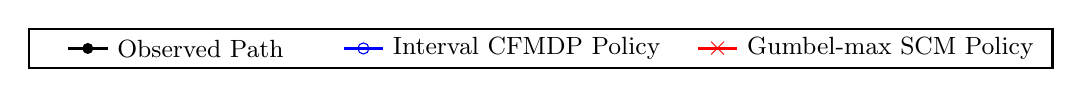
\begin{tikzpicture}[scale=1.0, every node/.style={scale=1.0}]
            \draw[thick, black] (-3, -0.25) rectangle (10, 0.25);
            %
            \draw[black, line width=1pt] (-2.5, 0.0) -- (-2,0.0);
            \fill[black] (-2.25,0.0) circle (2pt); %
            \node[right] at (-2,0.0) {\small Observed Path};
            
            %
            \draw[blue, line width=1pt] (1.0,0.0) -- (1.5,0.0);
            \node[draw=blue, circle, minimum size=4pt, inner sep=0pt] at (1.25,0.0) {}; %
            \node[right] at (1.5,0.0) {\small Interval CFMDP Policy};
            
            %
            \draw[red, line width=1pt] (5.5,0) -- (6,0);
            \node[red] at (5.75,0) {$\boldsymbol{\times}$}; %
            \node[right] at (6,0) {\small Gumbel-max SCM Policy};
        \end{tikzpicture}
    }\\
    %
    \subfigure[\footnotesize Lowest cumulative reward: Interval CFMDP ($312$), Gumbel-max SCM ($312$)]{%
        \resizebox{0.76\columnwidth}{!}{
             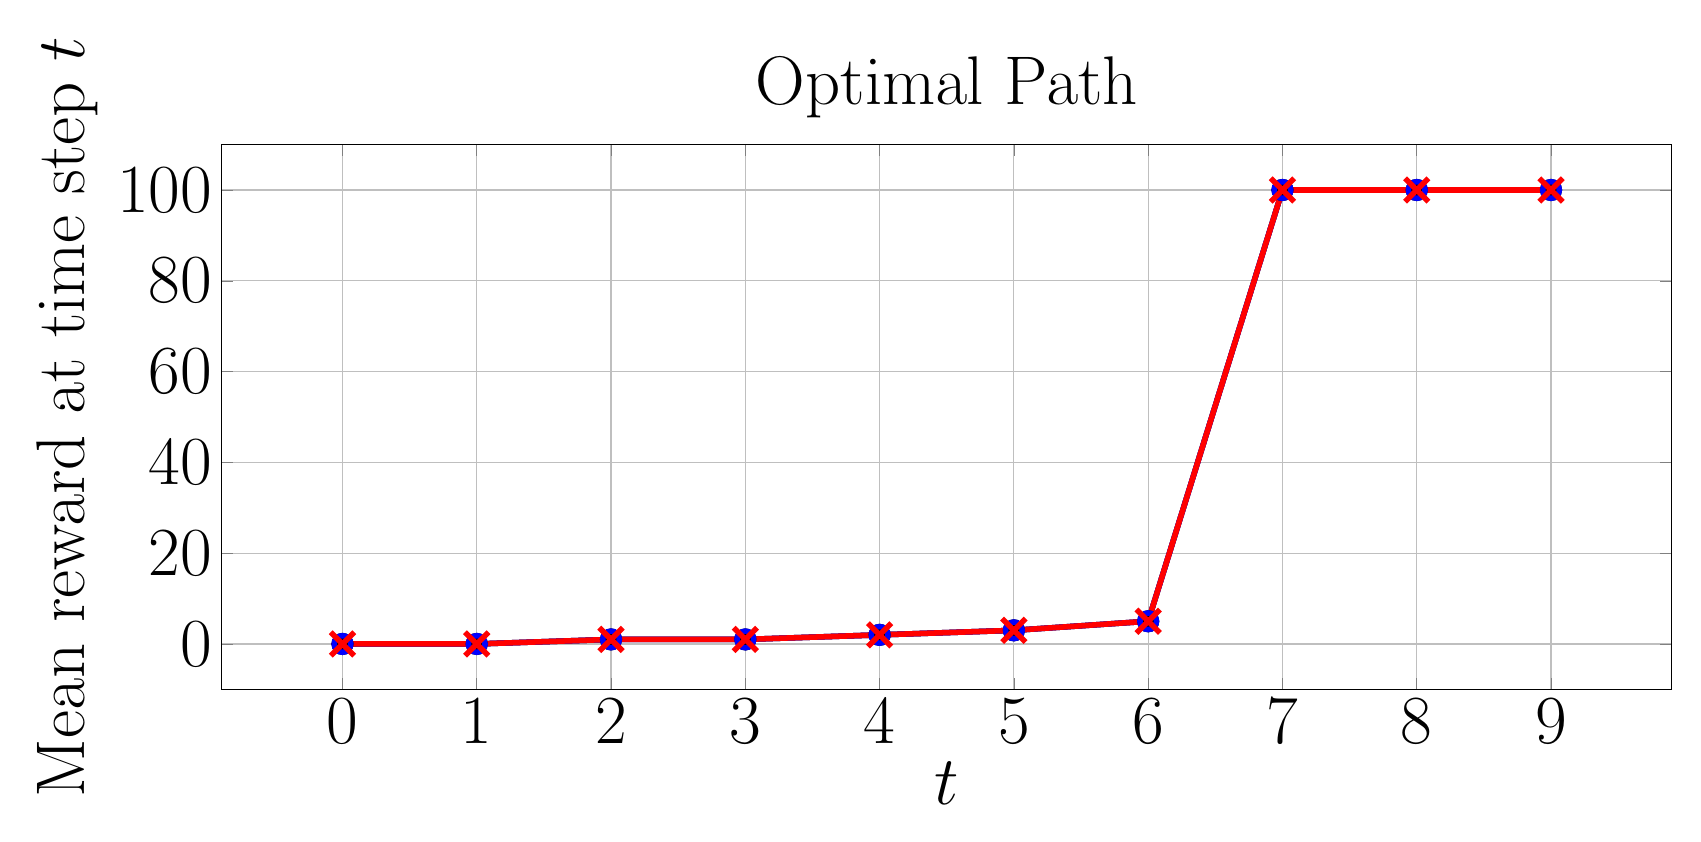
\begin{tikzpicture}
                \begin{axis}[
                    xlabel={$t$},
                    ylabel={Mean reward at time step $t$},
                    title={Optimal Path},
                    grid=both,
                    width=20cm, height=8.5cm,
                    every axis/.style={font=\Huge},
                    %
                ]
                \addplot[
                    color=black, %
                    mark=*, %
                    line width=2pt,
                    mark size=3pt,
                    error bars/.cd,
                    y dir=both, %
                    y explicit, %
                    error bar style={line width=1pt,solid},
                    error mark options={line width=1pt,mark size=4pt,rotate=90}
                ]
                coordinates {
                    (0, 0.0)  +- (0, 0.0)
                    (1, 0.0)  +- (0, 0.0) 
                    (2, 1.0)  +- (0, 0.0) 
                    (3, 1.0)  +- (0, 0.0)
                    (4, 2.0)  +- (0, 0.0)
                    (5, 3.0) +- (0, 0.0)
                    (6, 5.0) +- (0, 0.0)
                    (7, 100.0) +- (0, 0.0)
                    (8, 100.0) +- (0, 0.0)
                    (9, 100.0) +- (0, 0.0)
                };
                %
                \addplot[
                    color=blue, %
                    mark=o, %
                    line width=2pt,
                    mark size=3pt,
                    error bars/.cd,
                    y dir=both, %
                    y explicit, %
                    error bar style={line width=1pt,solid},
                    error mark options={line width=1pt,mark size=4pt,rotate=90}
                ]
                 coordinates {
                    (0, 0.0)  +- (0, 0.0)
                    (1, 0.0)  +- (0, 0.0) 
                    (2, 1.0)  +- (0, 0.0) 
                    (3, 1.0)  +- (0, 0.0)
                    (4, 2.0)  +- (0, 0.0)
                    (5, 3.0) +- (0, 0.0)
                    (6, 5.0) +- (0, 0.0)
                    (7, 100.0) +- (0, 0.0)
                    (8, 100.0) +- (0, 0.0)
                    (9, 100.0) +- (0, 0.0)
                };
                %
                \addplot[
                    color=red, %
                    mark=x, %
                    line width=2pt,
                    mark size=6pt,
                    error bars/.cd,
                    y dir=both, %
                    y explicit, %
                    error bar style={line width=1pt,solid},
                    error mark options={line width=1pt,mark size=4pt,rotate=90}
                ]
                coordinates {
                    (0, 0.0)  +- (0, 0.0)
                    (1, 0.0)  +- (0, 0.0) 
                    (2, 1.0)  +- (0, 0.0) 
                    (3, 1.0)  +- (0, 0.0)
                    (4, 2.0)  +- (0, 0.0)
                    (5, 3.0) +- (0, 0.0)
                    (6, 5.0) +- (0, 0.0)
                    (7, 100.0) +- (0, 0.0)
                    (8, 100.0) +- (0, 0.0)
                    (9, 100.0) +- (0, 0.0)
                };
                \end{axis}
            \end{tikzpicture}
         }
    }
    \hspace{1cm}
    \subfigure[\footnotesize Lowest cumulative reward: Interval CFMDP ($19$), Gumbel-max SCM ($-88$)]{%
         \resizebox{0.76\columnwidth}{!}{
            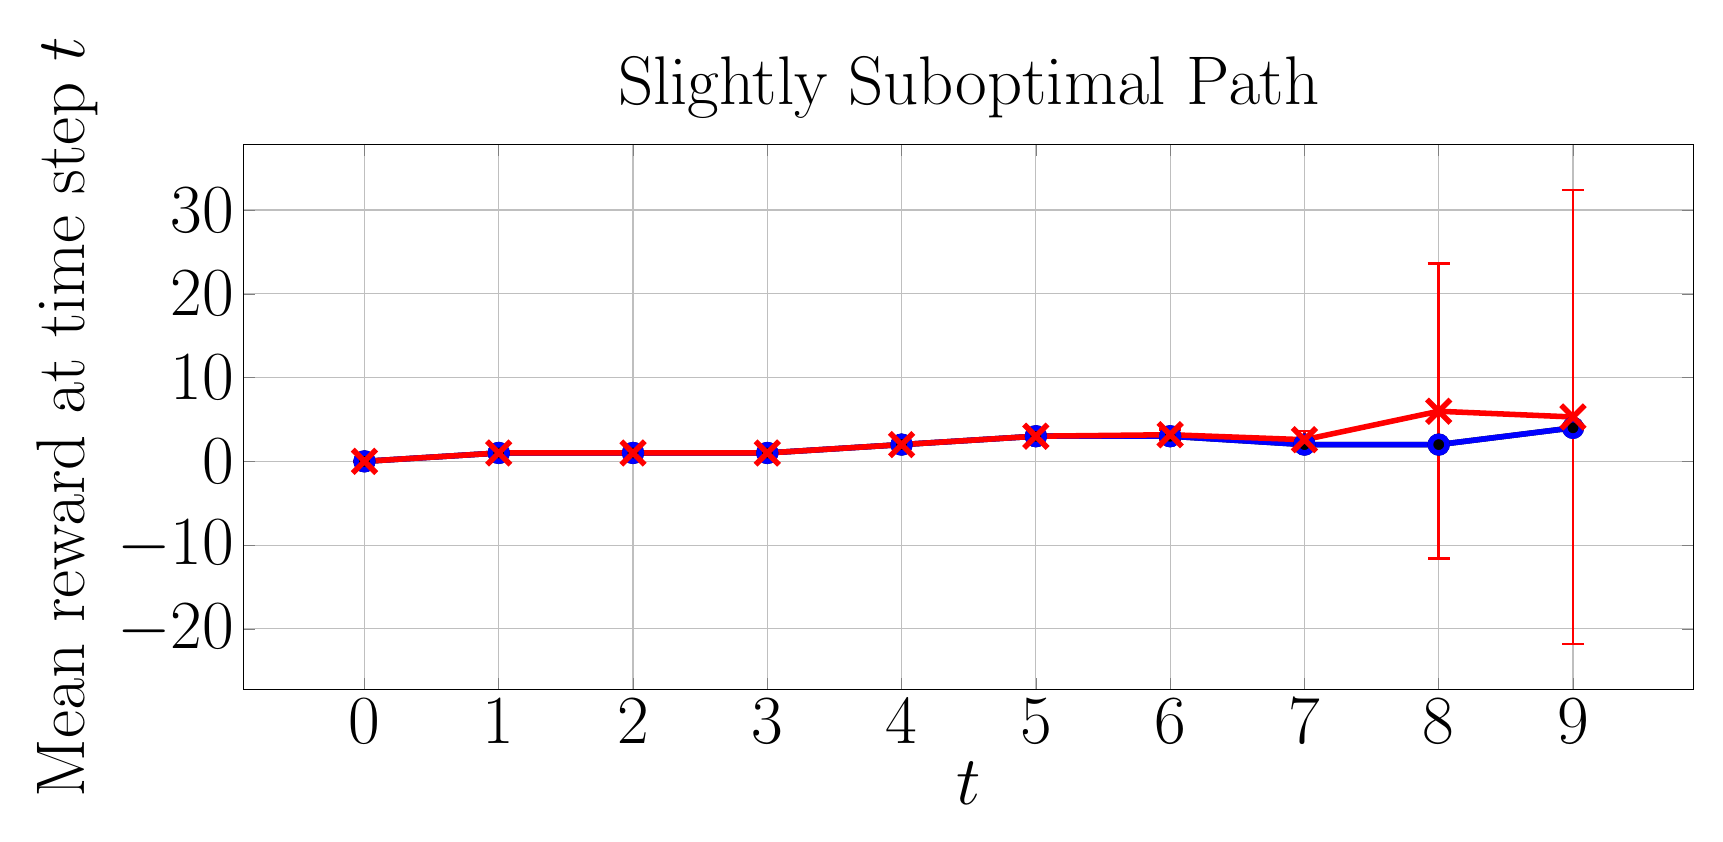
\begin{tikzpicture}
                \begin{axis}[
                    xlabel={$t$},
                    ylabel={Mean reward at time step $t$},
                    title={Slightly Suboptimal Path},
                    grid=both,
                    width=20cm, height=8.5cm,
                    every axis/.style={font=\Huge},
                    %
                ]
                \addplot[
                    color=black, %
                    mark=*, %
                    line width=2pt,
                    mark size=3pt,
                    error bars/.cd,
                    y dir=both, %
                    y explicit, %
                    error bar style={line width=1pt,solid},
                    error mark options={line width=1pt,mark size=4pt,rotate=90}
                ]
              coordinates {
                    (0, 0.0)  +- (0, 0.0)
                    (1, 1.0)  +- (0, 0.0) 
                    (2, 1.0)  +- (0, 0.0) 
                    (3, 1.0)  +- (0, 0.0)
                    (4, 2.0)  +- (0, 0.0)
                    (5, 3.0) +- (0, 0.0)
                    (6, 3.0) +- (0, 0.0)
                    (7, 2.0) +- (0, 0.0)
                    (8, 2.0) +- (0, 0.0)
                    (9, 4.0) +- (0, 0.0)
                };
                %
                \addplot[
                    color=blue, %
                    mark=o, %
                    line width=2pt,
                    mark size=3pt,
                    error bars/.cd,
                    y dir=both, %
                    y explicit, %
                    error bar style={line width=1pt,solid},
                    error mark options={line width=1pt,mark size=4pt,rotate=90}
                ]
              coordinates {
                    (0, 0.0)  +- (0, 0.0)
                    (1, 1.0)  +- (0, 0.0) 
                    (2, 1.0)  +- (0, 0.0) 
                    (3, 1.0)  +- (0, 0.0)
                    (4, 2.0)  +- (0, 0.0)
                    (5, 3.0) +- (0, 0.0)
                    (6, 3.0) +- (0, 0.0)
                    (7, 2.0) +- (0, 0.0)
                    (8, 2.0) +- (0, 0.0)
                    (9, 4.0) +- (0, 0.0)
                };
                %
                \addplot[
                    color=red, %
                    mark=x, %
                    line width=2pt,
                    mark size=6pt,
                    error bars/.cd,
                    y dir=both, %
                    y explicit, %
                    error bar style={line width=1pt,solid},
                    error mark options={line width=1pt,mark size=4pt,rotate=90}
                ]
                coordinates {
                    (0, 0.0)  +- (0, 0.0)
                    (1, 1.0)  +- (0, 0.0) 
                    (2, 1.0)  +- (0, 0.0) 
                    (3, 1.0)  +- (0, 0.0)
                    (4, 2.0)  += (0, 0.0)
                    (5, 3.0)  += (0, 0.0)
                    (6, 3.17847) += (0, 0.62606746) -= (0, 0.62606746)
                    (7, 2.5832885) += (0, 1.04598233) -= (0, 1.04598233)
                    (8, 5.978909) += (0, 17.60137623) -= (0, 17.60137623)
                    (9, 5.297059) += (0, 27.09227512) -= (0, 27.09227512)
                };
                \end{axis}
            \end{tikzpicture}
         }
    }\\[-1.5pt]
    \subfigure[\footnotesize Lowest cumulative reward: Interval CFMDP ($14$), Gumbel-max SCM ($-598$)]{%
         \resizebox{0.76\columnwidth}{!}{
             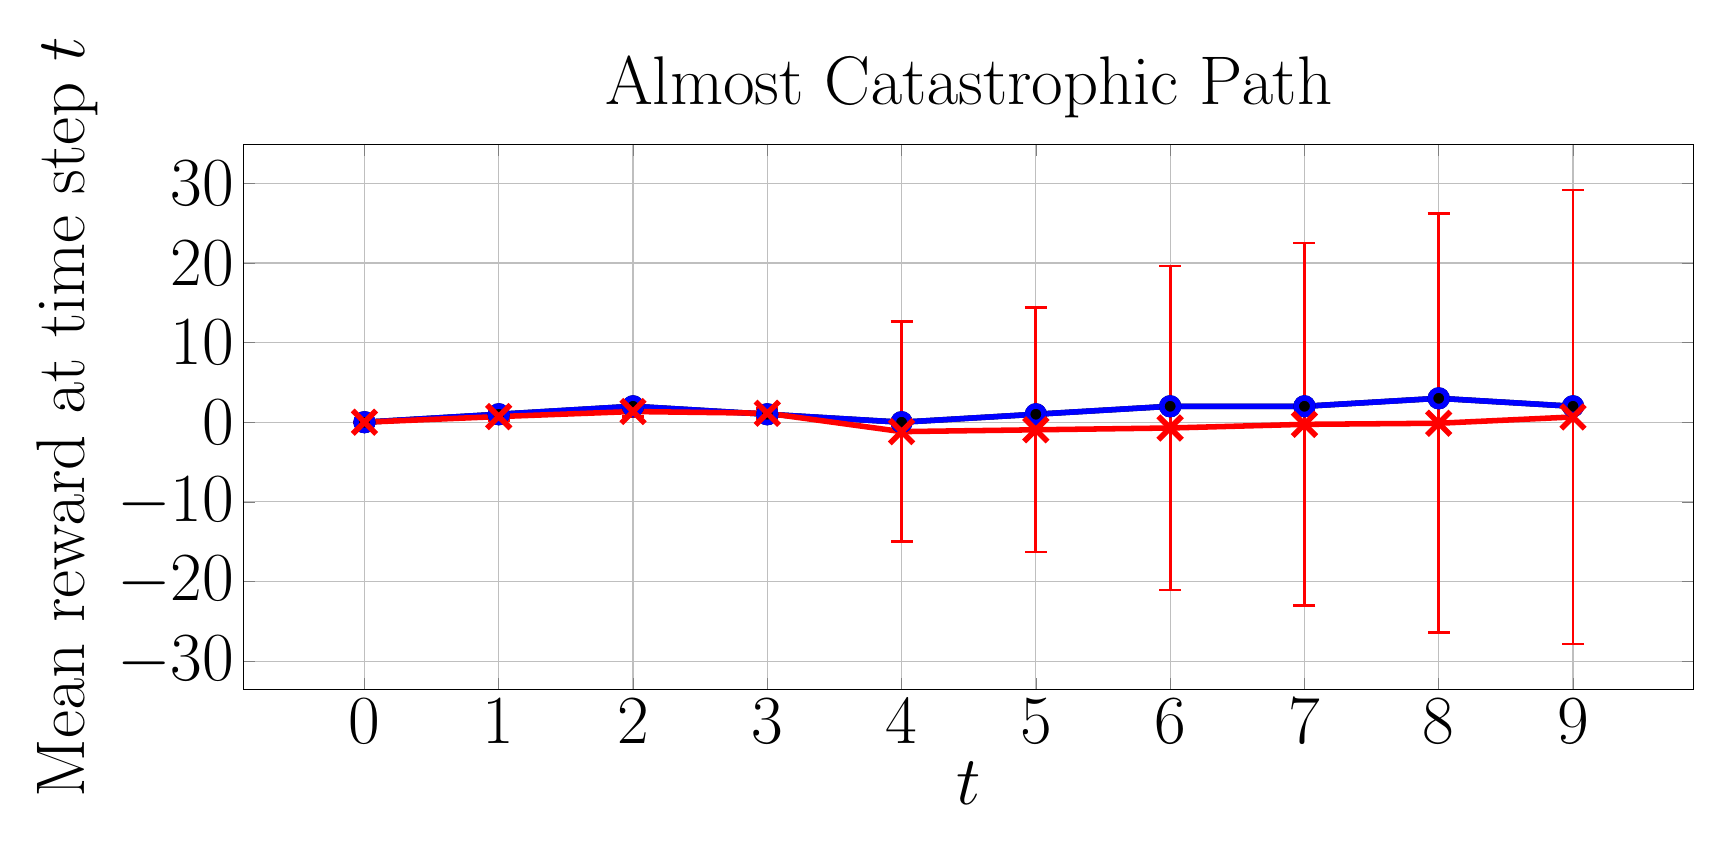
\begin{tikzpicture}
                \begin{axis}[
                    xlabel={$t$},
                    ylabel={Mean reward at time step $t$},
                    title={Almost Catastrophic Path},
                    grid=both,
                    width=20cm, height=8.5cm,
                    every axis/.style={font=\Huge},
                    %
                ]
                \addplot[
                    color=black, %
                    mark=*, %
                    line width=2pt,
                    mark size=3pt,
                    error bars/.cd,
                    y dir=both, %
                    y explicit, %
                    error bar style={line width=1pt,solid},
                    error mark options={line width=1pt,mark size=4pt,rotate=90}
                ]
                coordinates {
                    (0, 0.0)  +- (0, 0.0)
                    (1, 1.0)  +- (0, 0.0) 
                    (2, 2.0)  +- (0, 0.0) 
                    (3, 1.0)  +- (0, 0.0)
                    (4, 0.0)  +- (0, 0.0)
                    (5, 1.0) +- (0, 0.0)
                    (6, 2.0) +- (0, 0.0)
                    (7, 2.0) +- (0, 0.0)
                    (8, 3.0) +- (0, 0.0)
                    (9, 2.0) +- (0, 0.0)
                };
                %
                \addplot[
                    color=blue, %
                    mark=o, %
                    line width=2pt,
                    mark size=3pt,
                    error bars/.cd,
                    y dir=both, %
                    y explicit, %
                    error bar style={line width=1pt,solid},
                    error mark options={line width=1pt,mark size=4pt,rotate=90}
                ]
                coordinates {
                    (0, 0.0)  +- (0, 0.0)
                    (1, 1.0)  +- (0, 0.0) 
                    (2, 2.0)  +- (0, 0.0) 
                    (3, 1.0)  +- (0, 0.0)
                    (4, 0.0)  +- (0, 0.0)
                    (5, 1.0) +- (0, 0.0)
                    (6, 2.0) +- (0, 0.0)
                    (7, 2.0) +- (0, 0.0)
                    (8, 3.0) +- (0, 0.0)
                    (9, 2.0) +- (0, 0.0)
                };
                %
                \addplot[
                    color=red, %
                    mark=x, %
                    line width=2pt,
                    mark size=6pt,
                    error bars/.cd,
                    y dir=both, %
                    y explicit, %
                    error bar style={line width=1pt,solid},
                    error mark options={line width=1pt,mark size=4pt,rotate=90}
                ]
                coordinates {
                    (0, 0.0)  +- (0, 0.0)
                    (1, 0.7065655)  +- (0, 0.4553358) 
                    (2, 1.341673)  +- (0, 0.67091621) 
                    (3, 1.122926)  +- (0, 0.61281824)
                    (4, -1.1821935)  +- (0, 13.82444042)
                    (5, -0.952399)  +- (0, 15.35195457)
                    (6, -0.72672) +- (0, 20.33508414)
                    (7, -0.268983) +- (0, 22.77861454)
                    (8, -0.1310835) +- (0, 26.31013314)
                    (9, 0.65806) +- (0, 28.50670214)
                };
                %
            %
            %
            %
            %
            %
            %
            %
            %
            %
            %
            %
            %
            %
            %
            %
            %
            %
            %
                \end{axis}
            \end{tikzpicture}
         }
    }
    \hspace{1cm}
    \subfigure[\footnotesize Lowest cumulative reward: Interval CFMDP ($-698$), Gumbel-max SCM ($-698$)]{%
         \resizebox{0.76\columnwidth}{!}{
            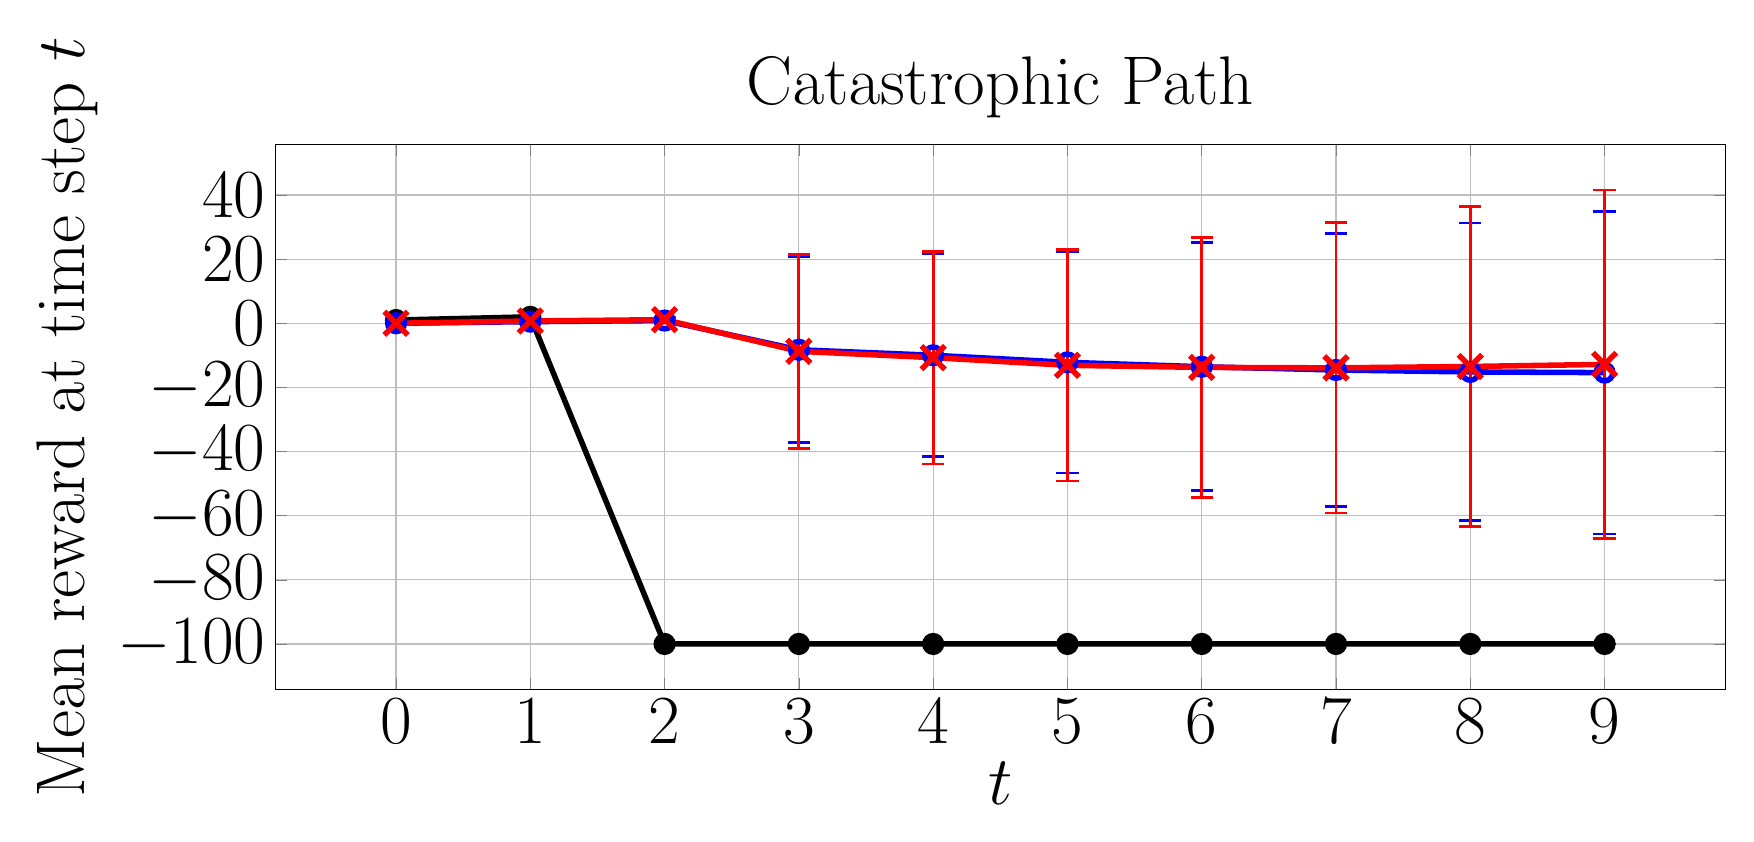
\begin{tikzpicture}
                \begin{axis}[
                    xlabel={$t$},
                    ylabel={Mean reward at time step $t$},
                    title={Catastrophic Path},
                    grid=both,
                    width=20cm, height=8.5cm,
                    every axis/.style={font=\Huge},
                    %
                ]
                \addplot[
                    color=black, %
                    mark=*, %
                    line width=2pt,
                    mark size=3pt,
                    error bars/.cd,
                    y dir=both, %
                    y explicit, %
                    error bar style={line width=1pt,solid},
                    error mark options={line width=1pt,mark size=4pt,rotate=90}
                ]
                coordinates {
                    (0, 1.0)  +- (0, 0.0)
                    (1, 2.0)  +- (0, 0.0) 
                    (2, -100.0)  +- (0, 0.0) 
                    (3, -100.0)  +- (0, 0.0)
                    (4, -100.0)  +- (0, 0.0)
                    (5, -100.0) +- (0, 0.0)
                    (6, -100.0) +- (0, 0.0)
                    (7, -100.0) +- (0, 0.0)
                    (8, -100.0) +- (0, 0.0)
                    (9, -100.0) +- (0, 0.0)
                };
                %
                \addplot[
                    color=blue, %
                    mark=o, %
                    line width=2pt,
                    mark size=3pt,
                    error bars/.cd,
                    y dir=both, %
                    y explicit, %
                    error bar style={line width=1pt,solid},
                    error mark options={line width=1pt,mark size=4pt,rotate=90}
                ]
                coordinates {
                    (0, 0.0)  +- (0, 0.0)
                    (1, 0.504814)  +- (0, 0.49997682) 
                    (2, 0.8439835)  +- (0, 0.76831917) 
                    (3, -8.2709165)  +- (0, 28.93656754)
                    (4, -9.981082)  +- (0, 31.66825363)
                    (5, -12.1776325) +- (0, 34.53463233)
                    (6, -13.556076) +- (0, 38.62845372)
                    (7, -14.574418) +- (0, 42.49603359)
                    (8, -15.1757075) +- (0, 46.41913968)
                    (9, -15.3900395) +- (0, 50.33563368)
                };
                %
                \addplot[
                    color=red, %
                    mark=x, %
                    line width=2pt,
                    mark size=6pt,
                    error bars/.cd,
                    y dir=both, %
                    y explicit, %
                    error bar style={line width=1pt,solid},
                    error mark options={line width=1pt,mark size=4pt,rotate=90}
                ]
                coordinates {
                    (0, 0.0)  +- (0, 0.0)
                    (1, 0.701873)  +- (0, 0.45743556) 
                    (2, 1.1227805)  +- (0, 0.73433129) 
                    (3, -8.7503255)  +- (0, 30.30257976)
                    (4, -10.722092)  +- (0, 33.17618589)
                    (5, -13.10721)  +- (0, 36.0648089)
                    (6, -13.7631645) +- (0, 40.56553451)
                    (7, -13.909043) +- (0, 45.23829402)
                    (8, -13.472517) +- (0, 49.96270296)
                    (9, -12.8278835) +- (0, 54.38618735)
                };
                %
            %
            %
            %
            %
            %
            %
            %
            %
            %
            %
            %
            %
            %
            %
            %
            %
            %
            %
                \end{axis}
            \end{tikzpicture}
         }
    }
    \caption{Average instant reward of CF paths induced by policies on GridWorld $p=0.4$.}
    \label{fig: reward p=0.4}
\end{figure*}

\subsection{Experimental Setup}
To compare policy performance, we measure the average rewards of counterfactual paths induced by our policy and the Gumbel-max policy by uniformly sampling $200$ counterfactual MDPs from the ICFMDP and generating $10,000$ counterfactual paths over each sampled CFMDP. \jl{Since the interval CFMDP depends on the observed path, we select $4$  paths of varying optimality to evaluate how the observed path impacts the performance of both policies: an optimal path, a slightly suboptimal path that could reach the optimal reward with a few changes, a catastrophic path that enters a catastrophic, terminal state with low reward, and an almost catastrophic path that was close to entering a catastrophic state.} When measuring the average probability bound widths and execution time needed to generate the ICFMDPs, we averaged over $20$ randomly generated observed paths
\footnote{Further training details are provided in Appendix \ref{app: training details}, and the code is provided at \href{https://github.com/ddv-lab/robust-cf-inference-in-MDPs}{https://github.com/ddv-lab/robust-cf-inference-in-MDPs}
%
%
.}.

\subsection{GridWorld}
\jl{The GridWorld MDP is a $4 \times 4$ grid where an agent must navigate from the top-left corner to the goal state in the bottom-right corner, avoiding a dangerous terminal state in the centre. At each time step, the agent can move up, down, left, or right, but there is a small probability (controlled by hyper-parameter $p$) of moving in an unintended direction. As the agent nears the goal, the reward for each state increases, culminating in a reward of $+100$ for reaching the goal. Entering the dangerous state results in a penalty of $-100$. We use two versions of GridWorld: a less stochastic version with $p=0.9$ (i.e., $90$\% chance of moving in the chosen direction) and a more stochastic version with $p=0.4$.}

\paragraph{GridWorld ($p=0.9$)}
When $p=0.9$, the counterfactual probability bounds are typically narrow (see Table \ref{tab:nonzero_probs} for average measurements). Consequently, as shown in Figure \ref{fig: reward p=0.9}, both policies are nearly identical and perform similarly well across the optimal, slightly suboptimal, and catastrophic paths.
%
However, for the almost catastrophic path, the interval CFMDP path is more conservative and follows the observed path more closely (as this is where the probability bounds are narrowest), which typically requires one additional step to reach the goal state than the Gumbel-max SCM policy.
%

\paragraph{GridWorld ($p=0.4$)}
\jl{When $p=0.4$, the GridWorld environment becomes more uncertain, increasing the risk of entering the dangerous state even if correct actions are chosen. Thus, as shown in Figure \ref{fig: reward p=0.4}, the interval CFMDP policy adopts a more conservative approach, avoiding deviation from the observed policy if it cannot guarantee higher counterfactual rewards (see the slightly suboptimal and almost catastrophic paths), whereas the Gumbel-max SCM is inconsistent: it can yield higher rewards, but also much lower rewards, reflected in the wide error bars.} For the catastrophic path, both policies must deviate from the observed path to achieve a higher reward and, in this case, perform similarly.
%
%
%
%
\subsection{Sepsis}
The Sepsis MDP \citep{oberst2019counterfactual} simulates trajectories of Sepsis patients. Each state consists of four vital signs (heart rate, blood pressure, oxygen concentration, and glucose levels), categorised as low, normal, or high.
and three treatments that can be toggled on/off at each time step (8 actions in total). Unlike \citet{oberst2019counterfactual}, we scale rewards based on the number of out-of-range vital signs, between $-1000$ (patient dies) and $1000$ (patient discharged). \jl{Like the GridWorld $p=0.4$ experiment, the Sepsis MDP is highly uncertain, as many states are equally likely to lead to optimal and poor outcomes. Thus, as shown in Figure \ref{fig: reward sepsis}, both policies follow the observed optimal and almost catastrophic paths to guarantee rewards are no worse than the observation.} However, improving the catastrophic path requires deviating from the observation. Here, the Gumbel-max SCM policy, on average, performs better than the interval CFMDP policy. But, since both policies have lower bounds clipped at $-1000$, neither policy reliably improves over the observation. In contrast, for the slightly suboptimal path, the interval CFMDP policy performs significantly better, shown by its higher lower bounds. 
Moreover, in these two cases, the worst-case counterfactual path generated by the interval CFMDP policy is better than that of the Gumbel-max SCM policy,
indicating its greater robustness.
%
\begin{figure*}
    \centering
     \resizebox{0.6\textwidth}{!}{
        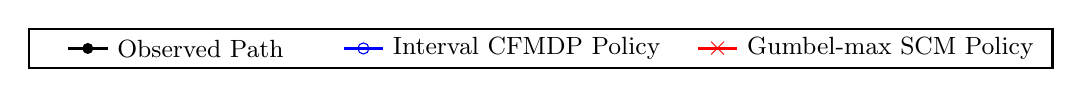
\begin{tikzpicture}[scale=1.0, every node/.style={scale=1.0}]
            \draw[thick, black] (-3, -0.25) rectangle (10, 0.25);
            %
            \draw[black, line width=1pt] (-2.5, 0.0) -- (-2,0.0);
            \fill[black] (-2.25,0.0) circle (2pt); %
            \node[right] at (-2,0.0) {\small Observed Path};
            
            %
            \draw[blue, line width=1pt] (1.0,0.0) -- (1.5,0.0);
            \node[draw=blue, circle, minimum size=4pt, inner sep=0pt] at (1.25,0.0) {}; %
            \node[right] at (1.5,0.0) {\small Interval CFMDP Policy};
            
            %
            \draw[red, line width=1pt] (5.5,0) -- (6,0);
            \node[red] at (5.75,0) {$\boldsymbol{\times}$}; %
            \node[right] at (6,0) {\small Gumbel-max SCM Policy};
        \end{tikzpicture}
    }\\
    \subfigure[\footnotesize Lowest cumulative reward: Interval CFMDP ($8000$), Gumbel-max SCM ($8000$)]{%
         \resizebox{0.76\columnwidth}{!}{
             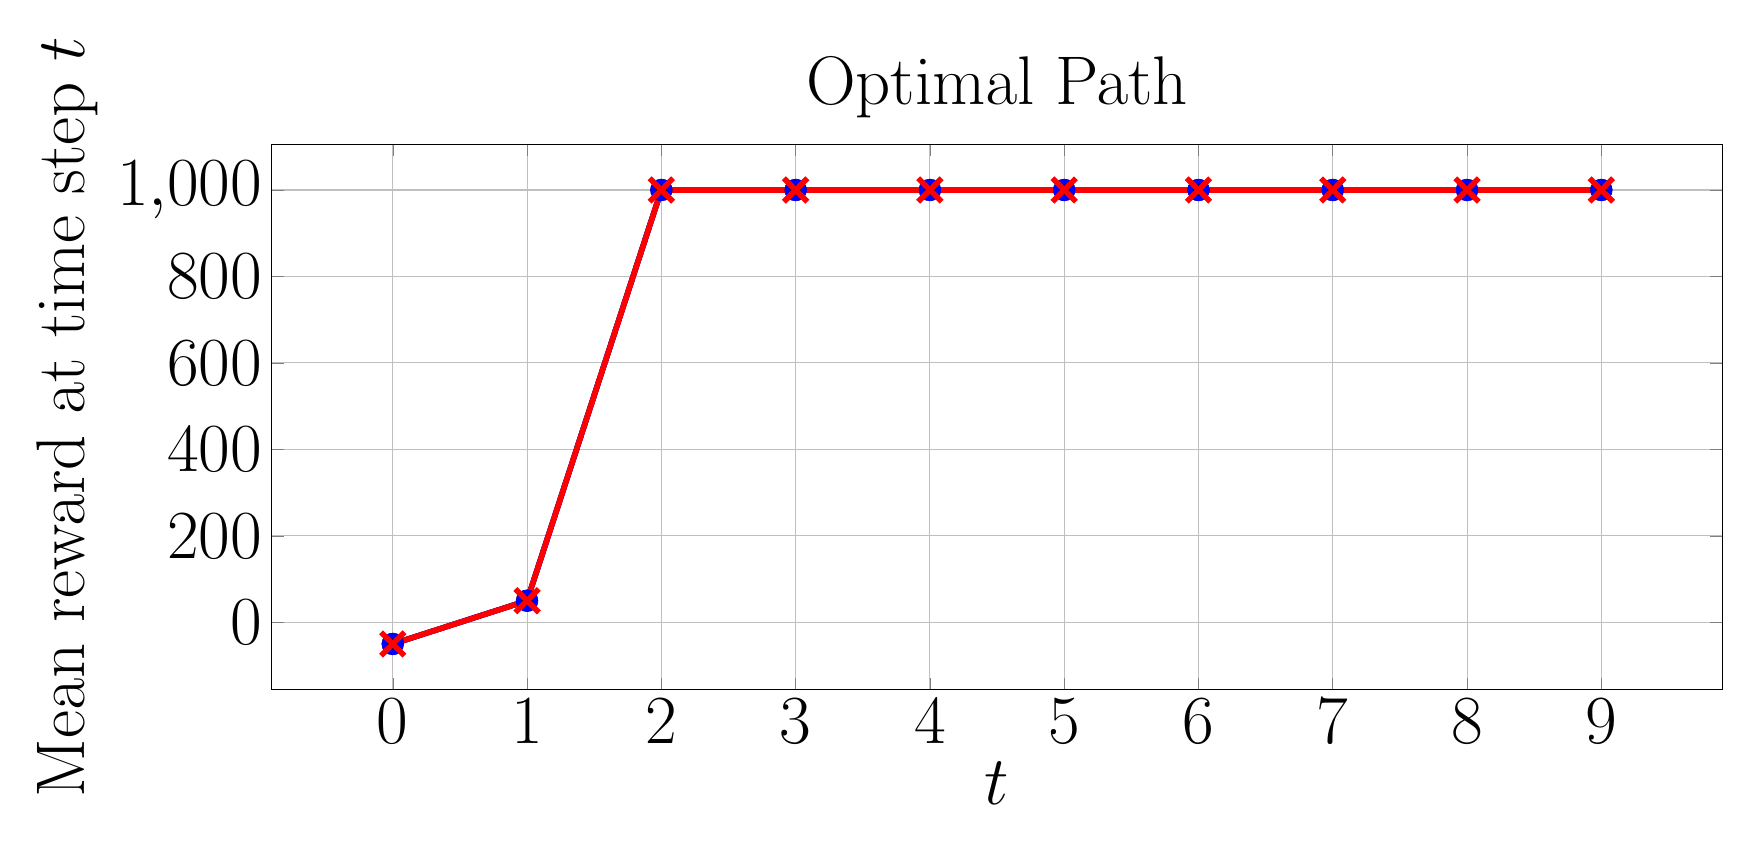
\begin{tikzpicture}
                \begin{axis}[
                    xlabel={$t$},
                    ylabel={Mean reward at time step $t$},
                    title={Optimal Path},
                    grid=both,
                    width=20cm, height=8.5cm,
                    every axis/.style={font=\Huge},
                    %
                ]
                \addplot[
                    color=black, %
                    mark=*, %
                    line width=2pt,
                    mark size=3pt,
                ]
                coordinates {
                    (0, -50.0)
                    (1, 50.0)
                    (2, 1000.0)
                    (3, 1000.0)
                    (4, 1000.0)
                    (5, 1000.0)
                    (6, 1000.0)
                    (7, 1000.0)
                    (8, 1000.0)
                    (9, 1000.0)
                };
                %
                \addplot[
                    color=blue, %
                    mark=o, %
                    line width=2pt,
                    mark size=3pt,
                    error bars/.cd,
                    y dir=both, %
                    y explicit, %
                    error bar style={line width=1pt,solid},
                    error mark options={line width=1pt,mark size=4pt,rotate=90}
                ]
                coordinates {
                    (0, -50.0)  +- (0, 0.0)
                    (1, 50.0)  +- (0, 0.0) 
                    (2, 1000.0)  +- (0, 0.0) 
                    (3, 1000.0)  +- (0, 0.0)
                    (4, 1000.0)  +- (0, 0.0)
                    (5, 1000.0) +- (0, 0.0)
                    (6, 1000.0) +- (0, 0.0)
                    (7, 1000.0) +- (0, 0.0)
                    (8, 1000.0) +- (0, 0.0)
                    (9, 1000.0) +- (0, 0.0)
                };
                %
                \addplot[
                    color=red, %
                    mark=x, %
                    line width=2pt,
                    mark size=6pt,
                    error bars/.cd,
                    y dir=both, %
                    y explicit, %
                    error bar style={line width=1pt,solid},
                    error mark options={line width=1pt,mark size=4pt,rotate=90}
                ]
                coordinates {
                    (0, -50.0)  +- (0, 0.0)
                    (1, 50.0)  +- (0, 0.0) 
                    (2, 1000.0)  +- (0, 0.0) 
                    (3, 1000.0)  +- (0, 0.0)
                    (4, 1000.0)  +- (0, 0.0)
                    (5, 1000.0) +- (0, 0.0)
                    (6, 1000.0) +- (0, 0.0)
                    (7, 1000.0) +- (0, 0.0)
                    (8, 1000.0) +- (0, 0.0)
                    (9, 1000.0) +- (0, 0.0)
                };
                %
                \end{axis}
            \end{tikzpicture}
         }
    }
    \hspace{1cm}
    \subfigure[\footnotesize Lowest cumulative reward: Interval CFMDP ($-5980$), Gumbel-max SCM ($-8000$)]{%
         \resizebox{0.76\columnwidth}{!}{
            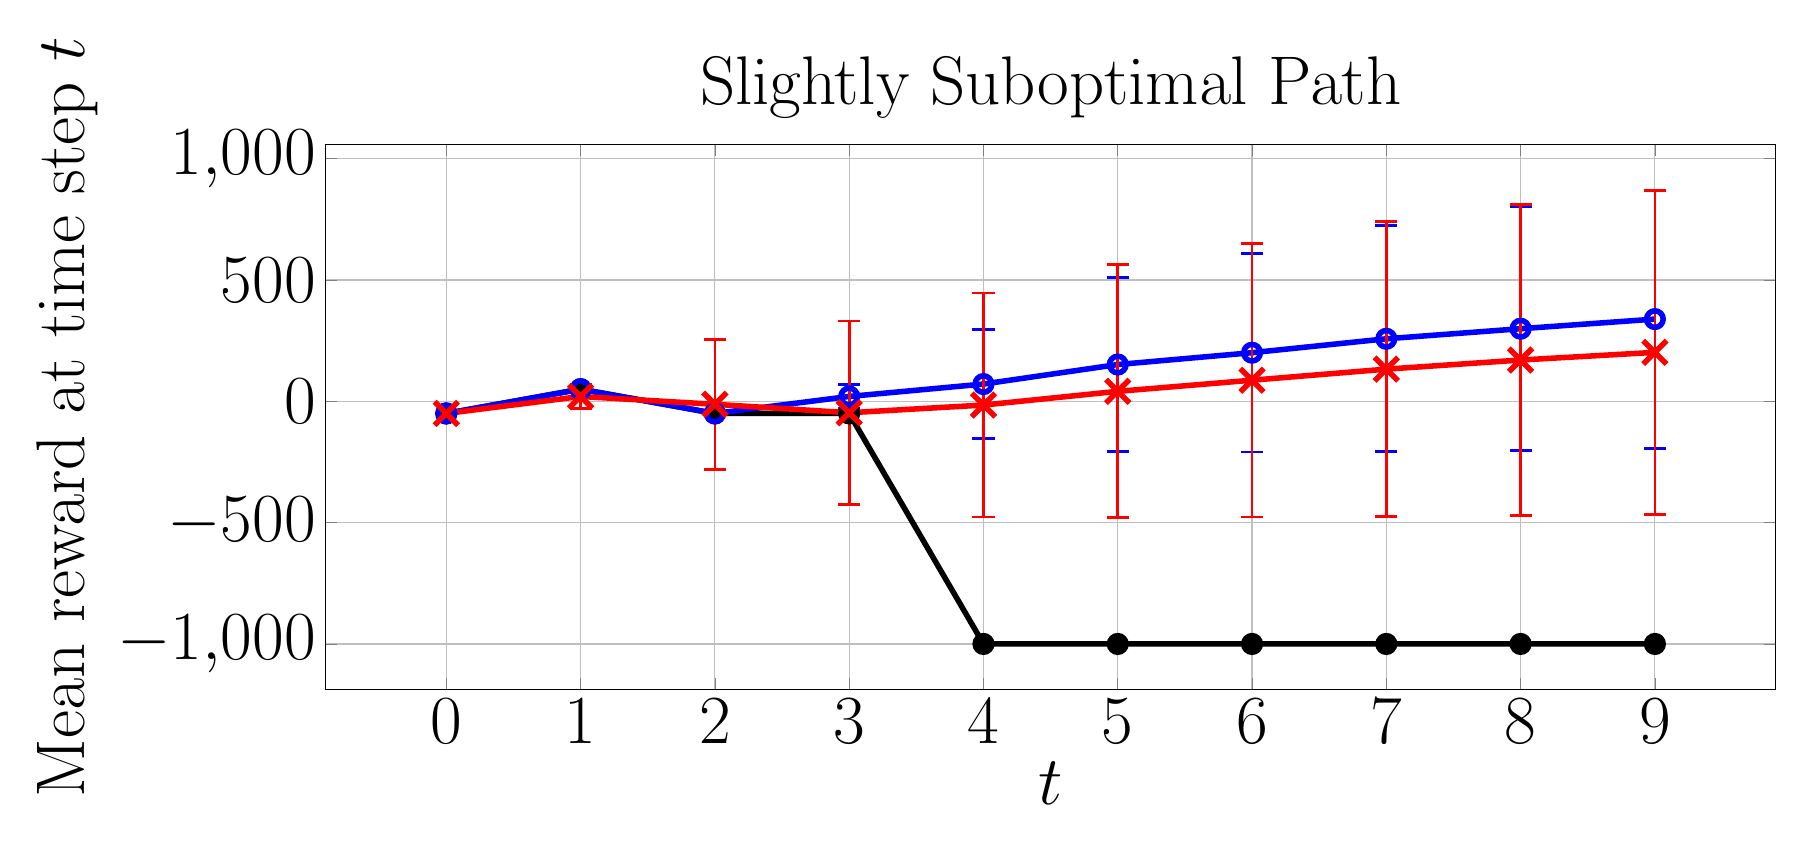
\begin{tikzpicture}
                \begin{axis}[
                    xlabel={$t$},
                    ylabel={Mean reward at time step $t$},
                    title={Slightly Suboptimal Path},
                    grid=both,
                    width=20cm, height=8.5cm,
                    every axis/.style={font=\Huge},
                    %
                ]
               \addplot[
                    color=black, %
                    mark=*, %
                    line width=2pt,
                    mark size=3pt,
                ]
                coordinates {
                    (0, -50.0)
                    (1, 50.0)
                    (2, -50.0)
                    (3, -50.0)
                    (4, -1000.0)
                    (5, -1000.0)
                    (6, -1000.0)
                    (7, -1000.0)
                    (8, -1000.0)
                    (9, -1000.0)
                };
                %
                \addplot[
                    color=blue, %
                    mark=o, %
                    line width=2pt,
                    mark size=3pt,
                    error bars/.cd,
                    y dir=both, %
                    y explicit, %
                    error bar style={line width=1pt,solid},
                    error mark options={line width=1pt,mark size=4pt,rotate=90}
                ]
                coordinates {
                    (0, -50.0)  +- (0, 0.0)
                    (1, 50.0)  +- (0, 0.0) 
                    (2, -50.0)  +- (0, 0.0) 
                    (3, 20.0631)  +- (0, 49.97539413)
                    (4, 71.206585)  +- (0, 226.02033693)
                    (5, 151.60797) +- (0, 359.23292559)
                    (6, 200.40593) +- (0, 408.86185176)
                    (7, 257.77948) +- (0, 466.10372804)
                    (8, 299.237465) +- (0, 501.82579506)
                    (9, 338.9129) +- (0, 532.06124996)
                };
                %
                \addplot[
                    color=red, %
                    mark=x, %
                    line width=2pt,
                    mark size=6pt,
                    error bars/.cd,
                    y dir=both, %
                    y explicit, %
                    error bar style={line width=1pt,solid},
                    error mark options={line width=1pt,mark size=4pt,rotate=90}
                ]
                coordinates {
                    (0, -50.0)  +- (0, 0.0)
                    (1, 20.00736)  +- (0, 49.99786741) 
                    (2, -12.282865)  +- (0, 267.598755) 
                    (3, -47.125995)  +- (0, 378.41755832)
                    (4, -15.381965)  +- (0, 461.77616558)
                    (5, 41.15459) +- (0, 521.53189262)
                    (6, 87.01595) +- (0, 564.22243126 )
                    (7, 132.62376) +- (0, 607.31338037)
                    (8, 170.168145) +- (0, 641.48013693)
                    (9, 201.813135) +- (0, 667.29441777)
                };
                %
                %
                %
                %
                %
                %
                %
                %
                %
                %
                %
                %
                %
                %
                %
                %
                %
                %
                %
                \end{axis}
            \end{tikzpicture}
         }
    }\\[-1.5pt]
    \subfigure[\footnotesize Lowest cumulative reward: Interval CFMDP ($100$), Gumbel-max SCM ($100$)]{%
         \resizebox{0.76\columnwidth}{!}{
             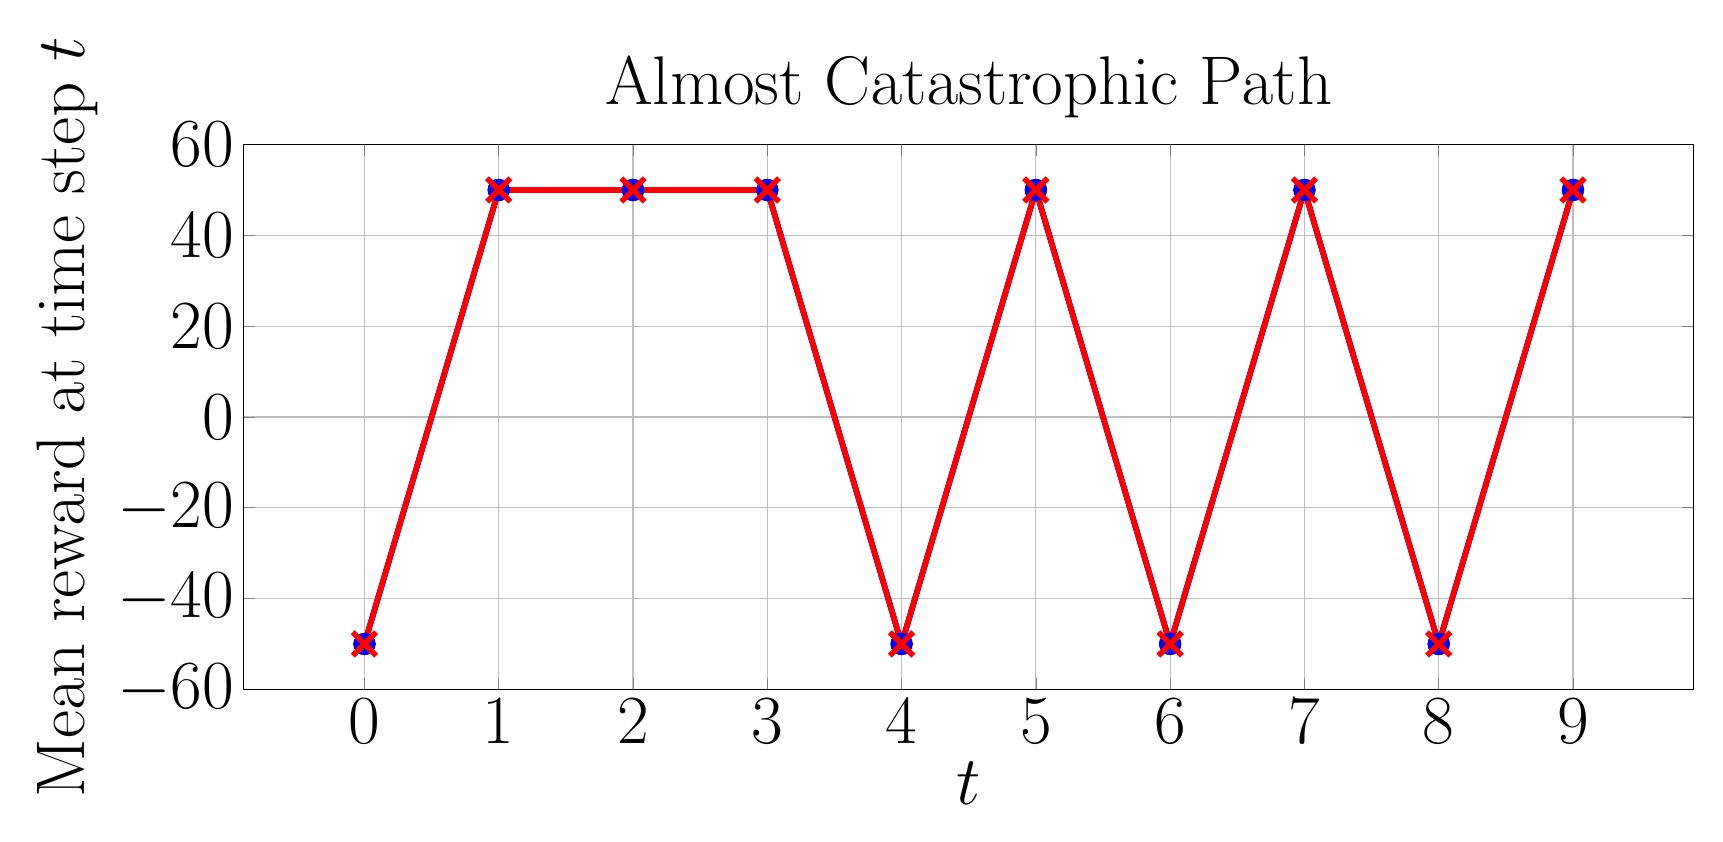
\begin{tikzpicture}
                \begin{axis}[
                    xlabel={$t$},
                    ylabel={Mean reward at time step $t$},
                    title={Almost Catastrophic Path},
                    grid=both,
                    every axis/.style={font=\Huge},
                    width=20cm, height=8.5cm,
                    %
                ]
               \addplot[
                    color=black, %
                    mark=*, %
                    line width=2pt,
                    mark size=3pt,
                ]
                coordinates {
                    (0, -50.0)
                    (1, 50.0)
                    (2, 50.0)
                    (3, 50.0)
                    (4, -50.0)
                    (5, 50.0)
                    (6, -50.0)
                    (7, 50.0)
                    (8, -50.0)
                    (9, 50.0)
                };
                %
                %
                \addplot[
                    color=blue, %
                    mark=o, %
                    line width=2pt,
                    mark size=3pt,
                    error bars/.cd,
                    y dir=both, %
                    y explicit, %
                    error bar style={line width=1pt,solid},
                    error mark options={line width=1pt,mark size=4pt,rotate=90}
                ]
                coordinates {
                    (0, -50.0)  +- (0, 0.0)
                    (1, 50.0)  +- (0, 0.0) 
                    (2, 50.0)  +- (0, 0.0) 
                    (3, 50.0)  +- (0, 0.0)
                    (4, -50.0)  +- (0, 0.0)
                    (5, 50.0) +- (0, 0.0)
                    (6, -50.0) +- (0, 0.0)
                    (7, 50.0) +- (0, 0.0)
                    (8, -50.0) +- (0, 0.0)
                    (9, 50.0) +- (0, 0.0)
                };
                %
                \addplot[
                    color=red, %
                    mark=x, %
                    line width=2pt,
                    mark size=6pt,
                    error bars/.cd,
                    y dir=both, %
                    y explicit, %
                    error bar style={line width=1pt,solid},
                    error mark options={line width=1pt,mark size=4pt,rotate=90}
                ]
                coordinates {
                    (0, -50.0)  +- (0, 0.0)
                    (1, 50.0)  +- (0, 0.0) 
                    (2, 50.0)  +- (0, 0.0) 
                    (3, 50.0)  +- (0, 0.0)
                    (4, -50.0)  +- (0, 0.0)
                    (5, 50.0) +- (0, 0.0)
                    (6, -50.0) +- (0, 0.0)
                    (7, 50.0) +- (0, 0.0)
                    (8, -50.0) +- (0, 0.0)
                    (9, 50.0) +- (0, 0.0)
                };
                %
                %
                %
                %
                %
                %
                %
                %
                %
                %
                %
                %
                %
                %
                %
                %
                %
                %
                %
                \end{axis}
            \end{tikzpicture}
         }
    }
    \hspace{1cm}
    \subfigure[\footnotesize Lowest cumulative reward: Interval CFMDP ($-7150$), Gumbel-max SCM ($-9050$)]{%
         \resizebox{0.76\columnwidth}{!}{
            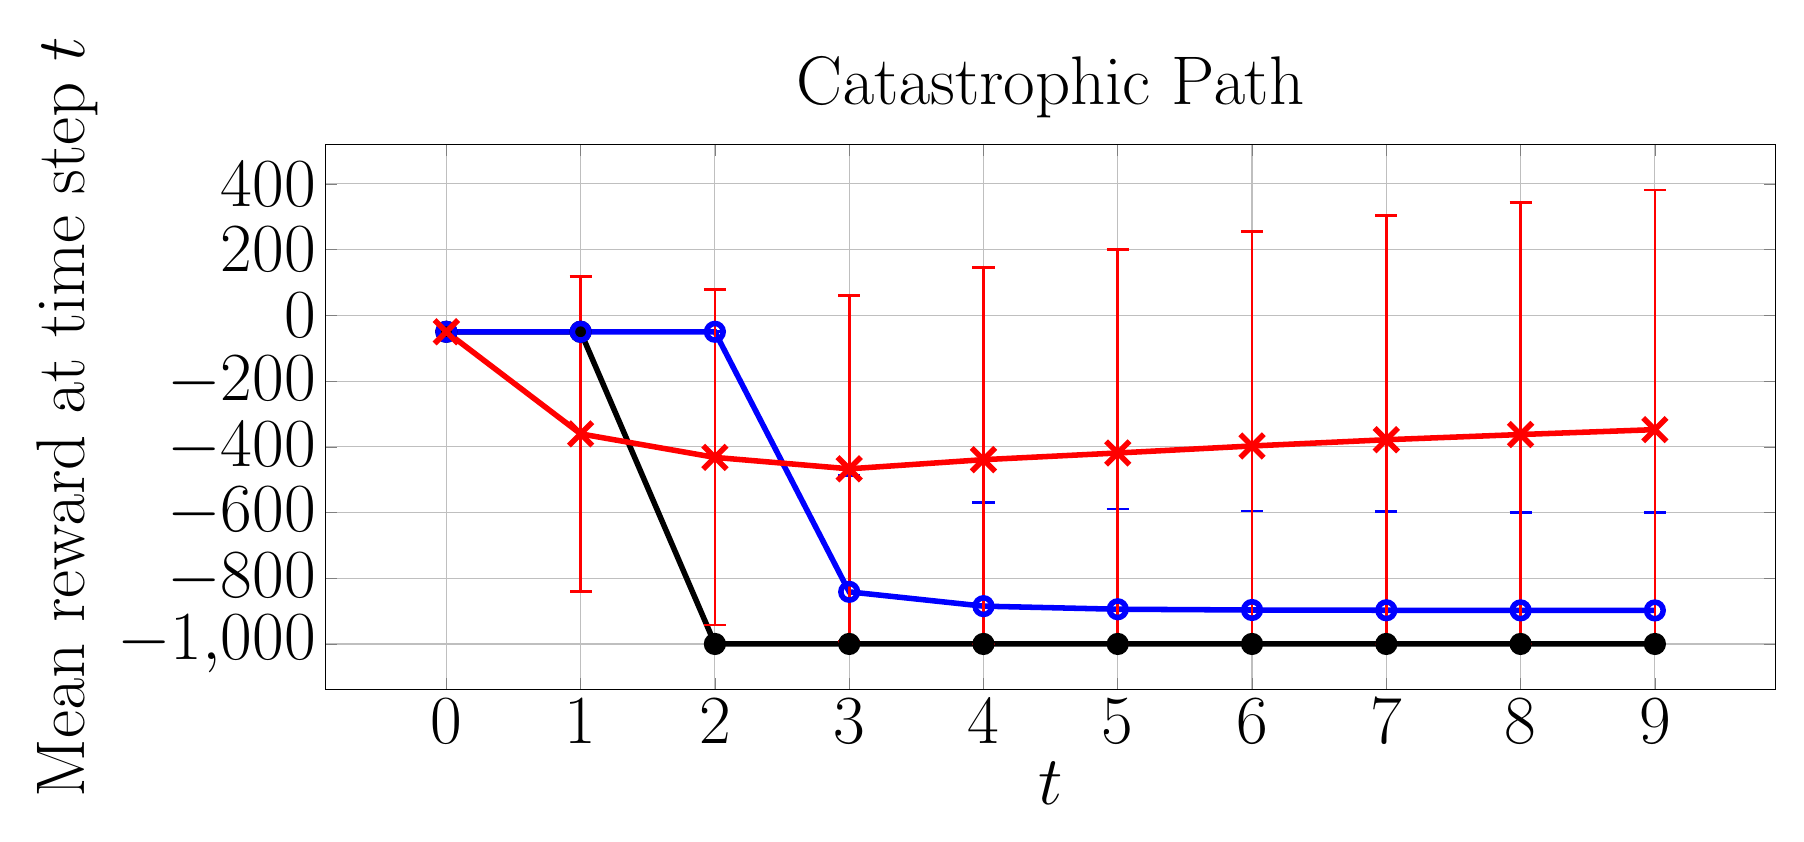
\begin{tikzpicture}
                \begin{axis}[
                    xlabel={$t$},
                    ylabel={Mean reward at time step $t$},
                    title={Catastrophic Path},
                    grid=both,
                    width=20cm, height=8.5cm,
                    every axis/.style={font=\Huge},
                    %
                ]
               \addplot[
                    color=black, %
                    mark=*, %
                    line width=2pt,
                    mark size=3pt,
                ]
                coordinates {
                    (0, -50.0)
                    (1, -50.0)
                    (2, -1000.0)
                    (3, -1000.0)
                    (4, -1000.0)
                    (5, -1000.0)
                    (6, -1000.0)
                    (7, -1000.0)
                    (8, -1000.0)
                    (9, -1000.0)
                };
                %
                %
                \addplot[
                    color=blue, %
                    mark=o, %
                    line width=2pt,
                    mark size=3pt,
                    error bars/.cd,
                    y dir=both, %
                    y explicit, %
                    error bar style={line width=1pt,solid},
                    error mark options={line width=1pt,mark size=4pt,rotate=90}
                ]
                coordinates {
                    (0, -50.0)  +- (0, 0.0)
                    (1, -50.0)  +- (0, 0.0) 
                    (2, -50.0)  +- (0, 0.0) 
                    (3, -841.440725)  += (0, 354.24605512) -= (0, 158.559275)
                    (4, -884.98225)  += (0, 315.37519669) -= (0, 115.01775)
                    (5, -894.330425) += (0, 304.88572805) -= (0, 105.669575)
                    (6, -896.696175) += (0, 301.19954514) -= (0, 103.303825)
                    (7, -897.4635) += (0, 299.61791279) -= (0, 102.5365)
                    (8, -897.77595) += (0, 298.80392585) -= (0, 102.22405)
                    (9, -897.942975) += (0, 298.32920557) -= (0, 102.057025)
                };
                %
                \addplot[
                    color=red, %
                    mark=x, %
                    line width=2pt,
                    mark size=6pt,
                    error bars/.cd,
                    y dir=both, %
                    y explicit, %
                    error bar style={line width=1pt,solid},
                    error mark options={line width=1pt,mark size=4pt,rotate=90}
                ]
            coordinates {
                    (0, -50.0)  +- (0, 0.0)
                    (1, -360.675265)  +- (0, 479.39812699) 
                    (2, -432.27629)  +- (0, 510.38620897) 
                    (3, -467.029545)  += (0, 526.36009628) -= (0, 526.36009628)
                    (4, -439.17429)  += (0, 583.96638919) -= (0, 560.82571)
                    (5, -418.82704) += (0, 618.43027478) -= (0, 581.17296)
                    (6, -397.464895) += (0, 652.67322574) -= (0, 602.535105)
                    (7, -378.49052) += (0, 682.85407033) -= (0, 621.50948)
                    (8, -362.654195) += (0, 707.01412023) -= (0, 637.345805)
                    (9, -347.737935) += (0, 729.29076479) -= (0, 652.262065)
                };
                %
                %
                %
                %
                %
                %
                %
                %
                %
                %
                %
                %
                %
                %
                %
                %
                %
                %
                %
                \end{axis}
            \end{tikzpicture}
         }
    }
    \caption{Average instant reward of CF paths induced by policies on Sepsis.}
    \label{fig: reward sepsis}
\end{figure*}

%
%
%
\subsection{Interval CFMDP Bounds}
%
%
Table \ref{tab:nonzero_probs} presents the mean counterfactual probability bound widths (excluding transitions where the upper bound is $0$) for each MDP, averaged over 20 observed paths. We compare the bounds under counterfactual stability (CS) and monotonicity (M) assumptions, CS alone, and no assumptions. This shows that the assumptions marginally reduce the bound widths, indicating the assumptions tighten the bounds without excluding too many causal models, as intended.
\renewcommand{\arraystretch}{1}

\begin{table}
\centering
\caption{Mean width of counterfactual probability bounds}
\resizebox{0.8\columnwidth}{!}{%
\begin{tabular}{|c|c|c|c|}
\hline
\multirow{2}{*}{\textbf{Environment}} & \multicolumn{3}{c|}{\textbf{Assumptions}} \\ \cline{2-4}
 & \textbf{CS + M} & \textbf{CS} & \textbf{None\tablefootnote{\jl{Equivalent to \citet{li2024probabilities}'s bounds (see Section \ref{sec: equivalence with Li}).}}} \\ \hline
\textbf{GridWorld} ($p=0.9$) & 0.0817 & 0.0977 & 0.100 \\ \hline
\textbf{GridWorld} ($p=0.4$) & 0.552  & 0.638  & 0.646 \\ \hline
\textbf{Sepsis} & 0.138 & 0.140 & 0.140 \\ \hline
\end{tabular}
}
\label{tab:nonzero_probs}
\end{table}


\subsection{Execution Times}
Table \ref{tab: times} compares the average time needed to generate the interval CFMDP vs.\ the Gumbel-max SCM CFMDP for 20 observations.
The GridWorld algorithms were run single-threaded, while the Sepsis experiments were run in parallel.
Generating the interval CFMDP is significantly faster as it uses exact analytical bounds, whereas the Gumbel-max CFMDP requires sampling from the Gumbel distribution to estimate counterfactual transition probabilities. \jl{Since constructing the counterfactual MDP models is the main bottleneck in both approaches, ours is more efficient overall and suitable for larger MDPs.}
\begin{table}
\centering
\caption{Mean execution time to generate CFMDPs}
\resizebox{0.99\columnwidth}{!}{%
\begin{tabular}{|c|c|c|}
\hline
\multirow{2}{*}{\textbf{Environment}} & \multicolumn{2}{c|}{\textbf{Mean Execution Time (s)}} \\ \cline{2-3} 
                                      & \textbf{Interval CFMDP} & \textbf{Gumbel-max CFMDP} \\ \hline
\textbf{GridWorld ($p=0.9$) }                  & 0.261                   & 56.1                      \\ \hline
\textbf{GridWorld ($p=0.4$)  }                 & 0.336                   & 54.5                      \\ \hline
\textbf{Sepsis}                                 & 688                     & 2940                      \\ \hline
\end{tabular}%
}
\label{tab: times}
\end{table}


\section{Related Work}
\label{Related Work}
\section{RELATED WORK}
\label{sec:relatedwork}
In this section, we describe the previous works related to our proposal, which are divided into two parts. In Section~\ref{sec:relatedwork_exoplanet}, we present a review of approaches based on machine learning techniques for the detection of planetary transit signals. Section~\ref{sec:relatedwork_attention} provides an account of the approaches based on attention mechanisms applied in Astronomy.\par

\subsection{Exoplanet detection}
\label{sec:relatedwork_exoplanet}
Machine learning methods have achieved great performance for the automatic selection of exoplanet transit signals. One of the earliest applications of machine learning is a model named Autovetter \citep{MCcauliff}, which is a random forest (RF) model based on characteristics derived from Kepler pipeline statistics to classify exoplanet and false positive signals. Then, other studies emerged that also used supervised learning. \cite{mislis2016sidra} also used a RF, but unlike the work by \citet{MCcauliff}, they used simulated light curves and a box least square \citep[BLS;][]{kovacs2002box}-based periodogram to search for transiting exoplanets. \citet{thompson2015machine} proposed a k-nearest neighbors model for Kepler data to determine if a given signal has similarity to known transits. Unsupervised learning techniques were also applied, such as self-organizing maps (SOM), proposed \citet{armstrong2016transit}; which implements an architecture to segment similar light curves. In the same way, \citet{armstrong2018automatic} developed a combination of supervised and unsupervised learning, including RF and SOM models. In general, these approaches require a previous phase of feature engineering for each light curve. \par

%DL is a modern data-driven technology that automatically extracts characteristics, and that has been successful in classification problems from a variety of application domains. The architecture relies on several layers of NNs of simple interconnected units and uses layers to build increasingly complex and useful features by means of linear and non-linear transformation. This family of models is capable of generating increasingly high-level representations \citep{lecun2015deep}.

The application of DL for exoplanetary signal detection has evolved rapidly in recent years and has become very popular in planetary science.  \citet{pearson2018} and \citet{zucker2018shallow} developed CNN-based algorithms that learn from synthetic data to search for exoplanets. Perhaps one of the most successful applications of the DL models in transit detection was that of \citet{Shallue_2018}; who, in collaboration with Google, proposed a CNN named AstroNet that recognizes exoplanet signals in real data from Kepler. AstroNet uses the training set of labelled TCEs from the Autovetter planet candidate catalog of Q1–Q17 data release 24 (DR24) of the Kepler mission \citep{catanzarite2015autovetter}. AstroNet analyses the data in two views: a ``global view'', and ``local view'' \citep{Shallue_2018}. \par


% The global view shows the characteristics of the light curve over an orbital period, and a local view shows the moment at occurring the transit in detail

%different = space-based

Based on AstroNet, researchers have modified the original AstroNet model to rank candidates from different surveys, specifically for Kepler and TESS missions. \citet{ansdell2018scientific} developed a CNN trained on Kepler data, and included for the first time the information on the centroids, showing that the model improves performance considerably. Then, \citet{osborn2020rapid} and \citet{yu2019identifying} also included the centroids information, but in addition, \citet{osborn2020rapid} included information of the stellar and transit parameters. Finally, \citet{rao2021nigraha} proposed a pipeline that includes a new ``half-phase'' view of the transit signal. This half-phase view represents a transit view with a different time and phase. The purpose of this view is to recover any possible secondary eclipse (the object hiding behind the disk of the primary star).


%last pipeline applies a procedure after the prediction of the model to obtain new candidates, this process is carried out through a series of steps that include the evaluation with Discovery and Validation of Exoplanets (DAVE) \citet{kostov2019discovery} that was adapted for the TESS telescope.\par
%



\subsection{Attention mechanisms in astronomy}
\label{sec:relatedwork_attention}
Despite the remarkable success of attention mechanisms in sequential data, few papers have exploited their advantages in astronomy. In particular, there are no models based on attention mechanisms for detecting planets. Below we present a summary of the main applications of this modeling approach to astronomy, based on two points of view; performance and interpretability of the model.\par
%Attention mechanisms have not yet been explored in all sub-areas of astronomy. However, recent works show a successful application of the mechanism.
%performance

The application of attention mechanisms has shown improvements in the performance of some regression and classification tasks compared to previous approaches. One of the first implementations of the attention mechanism was to find gravitational lenses proposed by \citet{thuruthipilly2021finding}. They designed 21 self-attention-based encoder models, where each model was trained separately with 18,000 simulated images, demonstrating that the model based on the Transformer has a better performance and uses fewer trainable parameters compared to CNN. A novel application was proposed by \citet{lin2021galaxy} for the morphological classification of galaxies, who used an architecture derived from the Transformer, named Vision Transformer (VIT) \citep{dosovitskiy2020image}. \citet{lin2021galaxy} demonstrated competitive results compared to CNNs. Another application with successful results was proposed by \citet{zerveas2021transformer}; which first proposed a transformer-based framework for learning unsupervised representations of multivariate time series. Their methodology takes advantage of unlabeled data to train an encoder and extract dense vector representations of time series. Subsequently, they evaluate the model for regression and classification tasks, demonstrating better performance than other state-of-the-art supervised methods, even with data sets with limited samples.

%interpretation
Regarding the interpretability of the model, a recent contribution that analyses the attention maps was presented by \citet{bowles20212}, which explored the use of group-equivariant self-attention for radio astronomy classification. Compared to other approaches, this model analysed the attention maps of the predictions and showed that the mechanism extracts the brightest spots and jets of the radio source more clearly. This indicates that attention maps for prediction interpretation could help experts see patterns that the human eye often misses. \par

In the field of variable stars, \citet{allam2021paying} employed the mechanism for classifying multivariate time series in variable stars. And additionally, \citet{allam2021paying} showed that the activation weights are accommodated according to the variation in brightness of the star, achieving a more interpretable model. And finally, related to the TESS telescope, \citet{morvan2022don} proposed a model that removes the noise from the light curves through the distribution of attention weights. \citet{morvan2022don} showed that the use of the attention mechanism is excellent for removing noise and outliers in time series datasets compared with other approaches. In addition, the use of attention maps allowed them to show the representations learned from the model. \par

Recent attention mechanism approaches in astronomy demonstrate comparable results with earlier approaches, such as CNNs. At the same time, they offer interpretability of their results, which allows a post-prediction analysis. \par



\section{Conclusion}
\label{Conclusion and Future Work}
\section{Conclusion}
In this work, we propose a simple yet effective approach, called SMILE, for graph few-shot learning with fewer tasks. Specifically, we introduce a novel dual-level mixup strategy, including within-task and across-task mixup, for enriching the diversity of nodes within each task and the diversity of tasks. Also, we incorporate the degree-based prior information to learn expressive node embeddings. Theoretically, we prove that SMILE effectively enhances the model's generalization performance. Empirically, we conduct extensive experiments on multiple benchmarks and the results suggest that SMILE significantly outperforms other baselines, including both in-domain and cross-domain few-shot settings.

\section*{Acknowledgements}
\label{Acknowledgements}
\section{Acknowledgements}


\appendices

\ifCLASSOPTIONcaptionsoff
  \newpage
\fi

\bibliographystyle{IEEEtran}
\bibliography{bibtext}

\begin{IEEEbiography}
[{\includegraphics[width=1in,height=1.25in,clip,keepaspectratio]{images/yvd5140.jpg}}]
{Yilu Dong}
is a Ph.D. student at Penn State University. He also 
received his M.S. and B.S. degrees from Penn State University. He is interested in communication protocols, software testing, and applied cryptography. His work focuses on the security of 5G systems. Specifically, improving the security and privacy of both UE and core network implementations. 
\end{IEEEbiography}

\begin{IEEEbiography} 
[{\includegraphics[width=1in,height=1.25in,clip,keepaspectratio]{images/rouzbeh_image.jpg}}]
{Rouzbeh Behnia}
is an assistant professor at the School of Information Systems and Management (SISM) at the University of South Florida. He received his Ph.D. in Computer Science from the University of South Florida.
His research focuses on different aspects of cybersecurity and applied cryptography. He is particularly interested in addressing privacy challenges in AI systems, developing post-quantum cryptographic solutions, and enhancing authentication protocols to ensure computation and communication integrity.
\end{IEEEbiography}

\begin{IEEEbiography}[{\includegraphics[width=1in,height=1.25in,clip,keepaspectratio]{images/AAY.jpg}}]{Attila A. Yavuz}
is an Associate Professor in the Department of Computer Science and Engineering and the Director of the Applied Cryptography Research Laboratory at the University of South Florida (USF). He was an Assistant Professor in the School of Electrical Engineering and Computer Science, at Oregon State University (2014-2018) and in the Department of Computer Science and Engineering, USF (2018-June 2021). He was a member of the security and privacy research group at the Robert Bosch Research and Technology Center North America (2011-2014). He received his Ph.D. degree in Computer Science from North Carolina State University (2011). He received his MS degree in Computer Science from Bogazici University (2006) in Istanbul, Turkey. He is broadly interested in the design, analysis, and application of cryptographic tools and protocols to enhance the security of computer systems. Attila Altay Yavuz is a recipient of the NSF CAREER Award, Cisco Research Award (thrice - 2019,2020,2022), and unrestricted research gifts from Robert Bosch (five times). He has authored over 100 products including research articles in top conferences, journals, and patents, some of which world-wide impact with actual deployments.
\end{IEEEbiography}

\begin{IEEEbiography}
[{\includegraphics[width=1in,height=1.25in,clip,keepaspectratio]{images/syed-rafiul-hussain-1.png}}]
{Syed Rafiul Hussain} (Member, IEEE) is an assistant professor in the Department of Computer Science and Engineering, Pennsylvania State University, State College, PA 16802 USA. His research interests include systems and network security, formal methods, program analysis and applied cryptography. He received a Ph.D. in computer science from Purdue University. He is a Member of IEEE and the Association for Computing Machinery.
\end{IEEEbiography}

\end{document}